\documentclass[twoside]{book}

% Packages required by doxygen
\usepackage{calc}
\usepackage{doxygen}
\usepackage{graphicx}
\usepackage[utf8]{inputenc}
\usepackage{makeidx}
\usepackage{multicol}
\usepackage{multirow}
\usepackage{textcomp}
\usepackage[table]{xcolor}

% Font selection
\usepackage[T1]{fontenc}
\usepackage{mathptmx}
\usepackage[scaled=.90]{helvet}
\usepackage{courier}
\usepackage{amssymb}
\usepackage{sectsty}
\renewcommand{\familydefault}{\sfdefault}
\allsectionsfont{%
  \fontseries{bc}\selectfont%
  \color{darkgray}%
}
\renewcommand{\DoxyLabelFont}{%
  \fontseries{bc}\selectfont%
  \color{darkgray}%
}

% Page & text layout
\usepackage{geometry}
\geometry{%
  a4paper,%
  top=2.5cm,%
  bottom=2.5cm,%
  left=2.5cm,%
  right=2.5cm%
}
\tolerance=750
\hfuzz=15pt
\hbadness=750
\setlength{\emergencystretch}{15pt}
\setlength{\parindent}{0cm}
\setlength{\parskip}{0.2cm}
\makeatletter
\renewcommand{\paragraph}{%
  \@startsection{paragraph}{4}{0ex}{-1.0ex}{1.0ex}{%
    \normalfont\normalsize\bfseries\SS@parafont%
  }%
}
\renewcommand{\subparagraph}{%
  \@startsection{subparagraph}{5}{0ex}{-1.0ex}{1.0ex}{%
    \normalfont\normalsize\bfseries\SS@subparafont%
  }%
}
\makeatother

% Headers & footers
\usepackage{fancyhdr}
\pagestyle{fancyplain}
\fancyhead[LE]{\fancyplain{}{\bfseries\thepage}}
\fancyhead[CE]{\fancyplain{}{}}
\fancyhead[RE]{\fancyplain{}{\bfseries\leftmark}}
\fancyhead[LO]{\fancyplain{}{\bfseries\rightmark}}
\fancyhead[CO]{\fancyplain{}{}}
\fancyhead[RO]{\fancyplain{}{\bfseries\thepage}}
\fancyfoot[LE]{\fancyplain{}{}}
\fancyfoot[CE]{\fancyplain{}{}}
\fancyfoot[RE]{\fancyplain{}{\bfseries\scriptsize Generated on Sat Dec 24 2016 22\-:54\-:49 for Mania++ by Doxygen }}
\fancyfoot[LO]{\fancyplain{}{\bfseries\scriptsize Generated on Sat Dec 24 2016 22\-:54\-:49 for Mania++ by Doxygen }}
\fancyfoot[CO]{\fancyplain{}{}}
\fancyfoot[RO]{\fancyplain{}{}}
\renewcommand{\footrulewidth}{0.4pt}
\renewcommand{\chaptermark}[1]{%
  \markboth{#1}{}%
}
\renewcommand{\sectionmark}[1]{%
  \markright{\thesection\ #1}%
}

% Indices & bibliography
\usepackage{natbib}
\usepackage[titles]{tocloft}
\setcounter{tocdepth}{3}
\setcounter{secnumdepth}{5}
\makeindex

% Hyperlinks (required, but should be loaded last)
\usepackage{ifpdf}
\ifpdf
  \usepackage[pdftex,pagebackref=true]{hyperref}
\else
  \usepackage[ps2pdf,pagebackref=true]{hyperref}
\fi
\hypersetup{%
  colorlinks=true,%
  linkcolor=blue,%
  citecolor=blue,%
  unicode%
}

% Custom commands
\newcommand{\clearemptydoublepage}{%
  \newpage{\pagestyle{empty}\cleardoublepage}%
}


%===== C O N T E N T S =====

\begin{document}

% Titlepage & ToC
\hypersetup{pageanchor=false}
\pagenumbering{roman}
\begin{titlepage}
\vspace*{7cm}
\begin{center}%
{\Large Mania++ }\\
\vspace*{1cm}
{\large Generated by Doxygen 1.8.6}\\
\vspace*{0.5cm}
{\small Sat Dec 24 2016 22:54:49}\\
\end{center}
\end{titlepage}
\clearemptydoublepage
\tableofcontents
\clearemptydoublepage
\pagenumbering{arabic}
\hypersetup{pageanchor=true}

%--- Begin generated contents ---
\chapter{Todo List}
\label{todo}
\hypertarget{todo}{}

\begin{DoxyRefList}
\item[\label{todo__todo000001}%
\hypertarget{todo__todo000001}{}%
Member \hyperlink{classCallBackManager_aecf87c2156353eb95b8ca85bebde8b71}{Call\-Back\-Manager\-:\-:Call\-Back\-Manager} (\hyperlink{classGbxRemote}{Gbx\-Remote} $\ast$server\-Ptr, \hyperlink{classCommandManager}{Command\-Manager} $\ast$command\-Manager\-Ptr, \hyperlink{classEventManager}{Event\-Manager} $\ast$event\-Manager\-Ptr, sql\-::\-Connection $\ast$database\-Ptr, std\-::map$<$ std\-::string, Player $>$ $\ast$player\-List, \hyperlink{classMapList}{Map\-List} $\ast$map\-List)]Replace pointer to \hyperlink{classGbxRemote}{Gbx\-Remote} with pointer to \hyperlink{classMethods}{Methods}. 
\item[\label{todo__todo000003}%
\hypertarget{todo__todo000003}{}%
Class \hyperlink{classGbxParameter}{Gbx\-Parameter} ]Handle structs.  
\item[\label{todo__todo000002}%
\hypertarget{todo__todo000002}{}%
Class \hyperlink{classGbxRemote}{Gbx\-Remote} ]Make it possible to set an A\-P\-I version without upsetting Tiny\-X\-M\-L2.  
\item[\label{todo__todo000005}%
\hypertarget{todo__todo000005}{}%
Member \hyperlink{classManiaPP_a18582fa28b259c22a8a8d526af62123a}{Mania\-P\-P\-:\-:retrieve\-Map\-List} ()]Insert map into database if needed.  
\item[\label{todo__todo000004}%
\hypertarget{todo__todo000004}{}%
Member \hyperlink{classManiaPP_aede94c0b982250de19186d447542e479}{Mania\-P\-P\-:\-:retrieve\-Player\-List} ()]Insert player into database if needed.  
\item[\label{todo__todo000006}%
\hypertarget{todo__todo000006}{}%
Member \hyperlink{classMethods_a0572ff430bc8be89035033fe17d8486a}{Methods\-:\-:Set\-Call\-Vote\-Ratios\-Ex} (bool replace\-All, std\-::vector$<$ Extended\-Call\-Vote\-Ratio $>$ ratios)]Implement when \hyperlink{classGbxParameters}{Gbx\-Parameters} supports structs. 
\end{DoxyRefList}
\chapter{Hierarchical Index}
\section{Class Hierarchy}
This inheritance list is sorted roughly, but not completely, alphabetically\-:\begin{DoxyCompactList}
\item \contentsline{section}{Call\-Back\-Manager}{\pageref{classCallBackManager}}{}
\item \contentsline{section}{Config}{\pageref{classConfig}}{}
\item \contentsline{section}{Controller}{\pageref{structController}}{}
\item \contentsline{section}{Database}{\pageref{classDatabase}}{}
\item \contentsline{section}{Database\-Config}{\pageref{structDatabaseConfig}}{}
\item \contentsline{section}{Entry\-Val}{\pageref{structEntryVal}}{}
\item \contentsline{section}{Event\-Manager}{\pageref{classEventManager}}{}
\item \contentsline{section}{Gbx\-Error}{\pageref{structGbxError}}{}
\item \contentsline{section}{Gbx\-First\-Response}{\pageref{structGbxFirstResponse}}{}
\item \contentsline{section}{Gbx\-Message}{\pageref{classGbxMessage}}{}
\item \contentsline{section}{Gbx\-Param}{\pageref{structGbxParam}}{}
\item \contentsline{section}{Gbx\-Parameter}{\pageref{classGbxParameter}}{}
\item \contentsline{section}{Gbx\-Parameters}{\pageref{classGbxParameters}}{}
\item \contentsline{section}{Gbx\-Query\-Response}{\pageref{structGbxQueryResponse}}{}
\item \contentsline{section}{Gbx\-Remote}{\pageref{classGbxRemote}}{}
\item \contentsline{section}{Gbx\-Response\-Parameter}{\pageref{classGbxResponseParameter}}{}
\item \contentsline{section}{Gbx\-Server\-Response}{\pageref{classGbxServerResponse}}{}
\begin{DoxyCompactList}
\item \contentsline{section}{Gbx\-Call\-Back}{\pageref{classGbxCallBack}}{}
\item \contentsline{section}{Gbx\-Response}{\pageref{classGbxResponse}}{}
\end{DoxyCompactList}
\item \contentsline{section}{Hex}{\pageref{classHex}}{}
\item \contentsline{section}{Logging}{\pageref{classLogging}}{}
\item \contentsline{section}{Mania\-P\-P}{\pageref{classManiaPP}}{}
\item \contentsline{section}{Map}{\pageref{structMap}}{}
\item \contentsline{section}{Map\-List}{\pageref{classMapList}}{}
\item \contentsline{section}{Methods}{\pageref{classMethods}}{}
\item \contentsline{section}{Player}{\pageref{structPlayer}}{}
\item \contentsline{section}{Player\-Ranking}{\pageref{structPlayerRanking}}{}
\item \contentsline{section}{Plugin}{\pageref{classPlugin}}{}
\item \contentsline{section}{Plugin\-Info}{\pageref{structPluginInfo}}{}
\item \contentsline{section}{Plugin\-Manager}{\pageref{classPluginManager}}{}
\item \contentsline{section}{Server\-Config}{\pageref{structServerConfig}}{}
\item \contentsline{section}{Server\-Status}{\pageref{structServerStatus}}{}
\item \contentsline{section}{Server\-Version}{\pageref{structServerVersion}}{}
\item \contentsline{section}{System\-Info}{\pageref{structSystemInfo}}{}
\item \contentsline{section}{Tcp\-Client}{\pageref{classTcpClient}}{}
\item \contentsline{section}{Time}{\pageref{classTime}}{}
\end{DoxyCompactList}

\chapter{Class Index}
\section{Class List}
Here are the classes, structs, unions and interfaces with brief descriptions\-:\begin{DoxyCompactList}
\item\contentsline{section}{\hyperlink{classCallBackManager}{Call\-Back\-Manager} \\*Handles callbacks from the server }{\pageref{classCallBackManager}}{}
\item\contentsline{section}{\hyperlink{structCallVoteRatio}{Call\-Vote\-Ratio} \\*Struct with a callvote ratio }{\pageref{structCallVoteRatio}}{}
\item\contentsline{section}{\hyperlink{classCommandManager}{Command\-Manager} \\*Manages the chat commands }{\pageref{classCommandManager}}{}
\item\contentsline{section}{\hyperlink{classConfig}{Config} \\*Reads and stores configuration information }{\pageref{classConfig}}{}
\item\contentsline{section}{\hyperlink{structController}{Controller} \\*Struct with all instances needed for plugins }{\pageref{structController}}{}
\item\contentsline{section}{\hyperlink{structCurrentCallVote}{Current\-Call\-Vote} \\*Struct with a current callvote }{\pageref{structCurrentCallVote}}{}
\item\contentsline{section}{\hyperlink{structCurrentNextValue}{Current\-Next\-Value} \\*Struct with a current and next value }{\pageref{structCurrentNextValue}}{}
\item\contentsline{section}{\hyperlink{classDatabase}{Database} \\*Handles the connection to the database }{\pageref{classDatabase}}{}
\item\contentsline{section}{\hyperlink{structDatabaseConfig}{Database\-Config} \\*\hyperlink{classDatabase}{Database} connection settings }{\pageref{structDatabaseConfig}}{}
\item\contentsline{section}{\hyperlink{structEntryVal}{Entry\-Val} \\*Struct with entry information }{\pageref{structEntryVal}}{}
\item\contentsline{section}{\hyperlink{classEventManager}{Event\-Manager} \\*Handles events (callbacks) from server to plugins }{\pageref{classEventManager}}{}
\item\contentsline{section}{\hyperlink{structExtendedCallVoteRatio}{Extended\-Call\-Vote\-Ratio} \\*Struct with a callvote }{\pageref{structExtendedCallVoteRatio}}{}
\item\contentsline{section}{\hyperlink{classGbxCallBack}{Gbx\-Call\-Back} \\*Call\-Back from server, de-\/\-X\-M\-L-\/fies the callback }{\pageref{classGbxCallBack}}{}
\item\contentsline{section}{\hyperlink{structGbxError}{Gbx\-Error} \\*Stores error details from the communication with the server }{\pageref{structGbxError}}{}
\item\contentsline{section}{\hyperlink{structGbxFirstResponse}{Gbx\-First\-Response} \\*Response received on handshake }{\pageref{structGbxFirstResponse}}{}
\item\contentsline{section}{\hyperlink{classGbxMessage}{Gbx\-Message} \\*X\-M\-L-\/fies the message for communication with the server }{\pageref{classGbxMessage}}{}
\item\contentsline{section}{\hyperlink{classGbxParameter}{Gbx\-Parameter} \\*X\-M\-L-\/fies the parameter for communication with the server }{\pageref{classGbxParameter}}{}
\item\contentsline{section}{\hyperlink{classGbxParameters}{Gbx\-Parameters} \\*List of parameters }{\pageref{classGbxParameters}}{}
\item\contentsline{section}{\hyperlink{structGbxQueryResponse}{Gbx\-Query\-Response} \\*Response received after a query is sent }{\pageref{structGbxQueryResponse}}{}
\item\contentsline{section}{\hyperlink{classGbxRemote}{Gbx\-Remote} \\*Handles communication with the Mania\-Planet server }{\pageref{classGbxRemote}}{}
\item\contentsline{section}{\hyperlink{classGbxResponse}{Gbx\-Response} \\*Response from server, de-\/\-X\-M\-L-\/fies the response }{\pageref{classGbxResponse}}{}
\item\contentsline{section}{\hyperlink{classGbxResponseParameter}{Gbx\-Response\-Parameter} \\*\hyperlink{structParameter}{Parameter} deducted from server response }{\pageref{classGbxResponseParameter}}{}
\item\contentsline{section}{\hyperlink{classGbxServerResponse}{Gbx\-Server\-Response} \\*Response from server, de-\/\-X\-M\-L-\/fies the response }{\pageref{classGbxServerResponse}}{}
\item\contentsline{section}{\hyperlink{classGbxStructParameters}{Gbx\-Struct\-Parameters} \\*List of struct parameters }{\pageref{classGbxStructParameters}}{}
\item\contentsline{section}{\hyperlink{structGitVersion}{Git\-Version} \\*Contains information about a Git release (version) }{\pageref{structGitVersion}}{}
\item\contentsline{section}{\hyperlink{classHex}{Hex} \\*Utility to print char arrays/pointers as hexadecimal values }{\pageref{classHex}}{}
\item\contentsline{section}{\hyperlink{classLogging}{Logging} \\*Utility to print information to the console }{\pageref{classLogging}}{}
\item\contentsline{section}{\hyperlink{structManiaLinkPageAnswer}{Mania\-Link\-Page\-Answer} \\*Struct with a Mania\-Link page answer }{\pageref{structManiaLinkPageAnswer}}{}
\item\contentsline{section}{\hyperlink{classManiaPP}{Mania\-P\-P} \\*Main class }{\pageref{classManiaPP}}{}
\item\contentsline{section}{\hyperlink{structMap}{Map} \\*Contains all information about a map in easy-\/to-\/use format }{\pageref{structMap}}{}
\item\contentsline{section}{\hyperlink{classMapList}{Map\-List} \\*Contains the maplist and a pointer to the current map }{\pageref{classMapList}}{}
\item\contentsline{section}{\hyperlink{classMethods}{Methods} \\*Contains all server methods and returns usable data types }{\pageref{classMethods}}{}
\item\contentsline{section}{\hyperlink{structParameter}{Parameter} \\*Pointer and type information of a parameter }{\pageref{structParameter}}{}
\item\contentsline{section}{\hyperlink{structPlayer}{Player} \\*Contains all information about a player in easy-\/to-\/use format }{\pageref{structPlayer}}{}
\item\contentsline{section}{\hyperlink{structPlayerRanking}{Player\-Ranking} \\*Struct with player ranking }{\pageref{structPlayerRanking}}{}
\item\contentsline{section}{\hyperlink{classPlugin}{Plugin} \\*\hyperlink{classPlugin}{Plugin} interface, inherited by all plugins }{\pageref{classPlugin}}{}
\item\contentsline{section}{\hyperlink{structPluginConfig}{Plugin\-Config} \\*\hyperlink{classPlugin}{Plugin} settings }{\pageref{structPluginConfig}}{}
\item\contentsline{section}{\hyperlink{classPluginHandler}{Plugin\-Handler} }{\pageref{classPluginHandler}}{}
\item\contentsline{section}{\hyperlink{structPluginInfo}{Plugin\-Info} \\*Struct with information about a plugin }{\pageref{structPluginInfo}}{}
\item\contentsline{section}{\hyperlink{classPluginManager}{Plugin\-Manager} \\*Manages the plugins }{\pageref{classPluginManager}}{}
\item\contentsline{section}{\hyperlink{structProgramConfig}{Program\-Config} \\*Program settings }{\pageref{structProgramConfig}}{}
\item\contentsline{section}{\hyperlink{structServerConfig}{Server\-Config} \\*Server connection settings }{\pageref{structServerConfig}}{}
\item\contentsline{section}{\hyperlink{structServerStatus}{Server\-Status} \\*Struct with server status }{\pageref{structServerStatus}}{}
\item\contentsline{section}{\hyperlink{structServerVersion}{Server\-Version} \\*Struct with server version information }{\pageref{structServerVersion}}{}
\item\contentsline{section}{\hyperlink{structSystemInfo}{System\-Info} \\*Struct with system information }{\pageref{structSystemInfo}}{}
\item\contentsline{section}{\hyperlink{classTcpClient}{Tcp\-Client} \\*Socket connection with server }{\pageref{classTcpClient}}{}
\item\contentsline{section}{\hyperlink{classText}{Text} \\*Contains utilities to format text }{\pageref{classText}}{}
\item\contentsline{section}{\hyperlink{classTime}{Time} \\*Contains utilities to format map times }{\pageref{classTime}}{}
\item\contentsline{section}{\hyperlink{structUIFrame}{U\-I\-Frame} \\*Mania\-Link for U\-I }{\pageref{structUIFrame}}{}
\item\contentsline{section}{\hyperlink{structUIList}{U\-I\-List} \\*Mania\-Link for U\-I list }{\pageref{structUIList}}{}
\item\contentsline{section}{\hyperlink{classUIManager}{U\-I\-Manager} \\*Manages the user interface on the server (Mania\-Links) }{\pageref{classUIManager}}{}
\item\contentsline{section}{\hyperlink{classVersionChecker}{Version\-Checker} \\*Checks Mania++ version (and possibly plugin versions) }{\pageref{classVersionChecker}}{}
\item\contentsline{section}{\hyperlink{classVersionCompare}{Version\-Compare} \\*Compares string versions }{\pageref{classVersionCompare}}{}
\end{DoxyCompactList}

\chapter{File Index}
\section{File List}
Here is a list of all files with brief descriptions\-:\begin{DoxyCompactList}
\item\contentsline{section}{/home/travis/build/\-The\-Maximum/mania-\/pp/src/\hyperlink{main_8cpp}{main.\-cpp} }{\pageref{main_8cpp}}{}
\item\contentsline{section}{/home/travis/build/\-The\-Maximum/mania-\/pp/src/\-Config/\hyperlink{Config_8cpp}{Config.\-cpp} }{\pageref{Config_8cpp}}{}
\item\contentsline{section}{/home/travis/build/\-The\-Maximum/mania-\/pp/src/\-Config/\hyperlink{Config_8h}{Config.\-h} }{\pageref{Config_8h}}{}
\item\contentsline{section}{/home/travis/build/\-The\-Maximum/mania-\/pp/src/\-Gbx\-Remote/\hyperlink{GbxMessage_8cpp}{Gbx\-Message.\-cpp} }{\pageref{GbxMessage_8cpp}}{}
\item\contentsline{section}{/home/travis/build/\-The\-Maximum/mania-\/pp/src/\-Gbx\-Remote/\hyperlink{GbxMessage_8h}{Gbx\-Message.\-h} }{\pageref{GbxMessage_8h}}{}
\item\contentsline{section}{/home/travis/build/\-The\-Maximum/mania-\/pp/src/\-Gbx\-Remote/\hyperlink{GbxParameter_8cpp}{Gbx\-Parameter.\-cpp} }{\pageref{GbxParameter_8cpp}}{}
\item\contentsline{section}{/home/travis/build/\-The\-Maximum/mania-\/pp/src/\-Gbx\-Remote/\hyperlink{GbxParameter_8h}{Gbx\-Parameter.\-h} }{\pageref{GbxParameter_8h}}{}
\item\contentsline{section}{/home/travis/build/\-The\-Maximum/mania-\/pp/src/\-Gbx\-Remote/\hyperlink{GbxParameters_8h}{Gbx\-Parameters.\-h} }{\pageref{GbxParameters_8h}}{}
\item\contentsline{section}{/home/travis/build/\-The\-Maximum/mania-\/pp/src/\-Gbx\-Remote/\hyperlink{GbxRemote_8cpp}{Gbx\-Remote.\-cpp} }{\pageref{GbxRemote_8cpp}}{}
\item\contentsline{section}{/home/travis/build/\-The\-Maximum/mania-\/pp/src/\-Gbx\-Remote/\hyperlink{GbxRemote_8h}{Gbx\-Remote.\-h} }{\pageref{GbxRemote_8h}}{}
\item\contentsline{section}{/home/travis/build/\-The\-Maximum/mania-\/pp/src/\-Gbx\-Remote/\hyperlink{GbxResponse_8cpp}{Gbx\-Response.\-cpp} }{\pageref{GbxResponse_8cpp}}{}
\item\contentsline{section}{/home/travis/build/\-The\-Maximum/mania-\/pp/src/\-Gbx\-Remote/\hyperlink{GbxResponse_8h}{Gbx\-Response.\-h} }{\pageref{GbxResponse_8h}}{}
\item\contentsline{section}{/home/travis/build/\-The\-Maximum/mania-\/pp/src/\-Gbx\-Remote/\hyperlink{GbxStructs_8h}{Gbx\-Structs.\-h} }{\pageref{GbxStructs_8h}}{}
\item\contentsline{section}{/home/travis/build/\-The\-Maximum/mania-\/pp/src/\-Socket/\hyperlink{TcpClient_8cpp}{Tcp\-Client.\-cpp} }{\pageref{TcpClient_8cpp}}{}
\item\contentsline{section}{/home/travis/build/\-The\-Maximum/mania-\/pp/src/\-Socket/\hyperlink{TcpClient_8h}{Tcp\-Client.\-h} }{\pageref{TcpClient_8h}}{}
\item\contentsline{section}{/home/travis/build/\-The\-Maximum/mania-\/pp/src/\-Utils/\hyperlink{Hex_8h}{Hex.\-h} }{\pageref{Hex_8h}}{}
\end{DoxyCompactList}

\chapter{Class Documentation}
\hypertarget{classConfig}{\section{Config Class Reference}
\label{classConfig}\index{Config@{Config}}
}


Reads and stores configuration information.  




{\ttfamily \#include $<$Config.\-h$>$}

\subsection*{Public Member Functions}
\begin{DoxyCompactItemize}
\item 
\hyperlink{classConfig_ae67e338ea42e242cb5b374b6583c8b1c}{Config} (std\-::string \hyperlink{classConfig_a08b7b2c4eadf7dda51404f76fd6e0280}{config\-File})
\begin{DoxyCompactList}\small\item\em Calls parse\-Config to parse the configuration file. \end{DoxyCompactList}\item 
\hyperlink{classConfig_a543dce59b66475c5108088ee4ce1cdfc}{$\sim$\-Config} ()
\end{DoxyCompactItemize}
\subsection*{Public Attributes}
\begin{DoxyCompactItemize}
\item 
\hypertarget{classConfig_a249a19a298cdcfd4223609142e15e5de}{\hyperlink{structServerConfig}{Server\-Config} $\ast$ \hyperlink{classConfig_a249a19a298cdcfd4223609142e15e5de}{Server}}\label{classConfig_a249a19a298cdcfd4223609142e15e5de}

\begin{DoxyCompactList}\small\item\em Instance of \hyperlink{structServerConfig}{Server\-Config} which stores the server connection settings. \end{DoxyCompactList}\item 
\hypertarget{classConfig_a7c1bdf72973da53666514dbd549cc400}{\hyperlink{structDatabaseConfig}{Database\-Config} $\ast$ \hyperlink{classConfig_a7c1bdf72973da53666514dbd549cc400}{Database}}\label{classConfig_a7c1bdf72973da53666514dbd549cc400}

\begin{DoxyCompactList}\small\item\em Instance of \hyperlink{structDatabaseConfig}{Database\-Config} which stores the database server connection settings. \end{DoxyCompactList}\end{DoxyCompactItemize}
\subsection*{Private Member Functions}
\begin{DoxyCompactItemize}
\item 
\hypertarget{classConfig_a2ddcecec4284da0fb0b53da77e0d217a}{void \hyperlink{classConfig_a2ddcecec4284da0fb0b53da77e0d217a}{parse\-Config} ()}\label{classConfig_a2ddcecec4284da0fb0b53da77e0d217a}

\begin{DoxyCompactList}\small\item\em Reads information from Y\-A\-M\-L file and puts this in configuration struct(s). \end{DoxyCompactList}\end{DoxyCompactItemize}
\subsection*{Private Attributes}
\begin{DoxyCompactItemize}
\item 
\hypertarget{classConfig_a08b7b2c4eadf7dda51404f76fd6e0280}{std\-::string \hyperlink{classConfig_a08b7b2c4eadf7dda51404f76fd6e0280}{config\-File}}\label{classConfig_a08b7b2c4eadf7dda51404f76fd6e0280}

\begin{DoxyCompactList}\small\item\em Name of the configuration file, set by constructor. \end{DoxyCompactList}\end{DoxyCompactItemize}


\subsection{Detailed Description}
Reads and stores configuration information. 

\subsection{Constructor \& Destructor Documentation}
\hypertarget{classConfig_ae67e338ea42e242cb5b374b6583c8b1c}{\index{Config@{Config}!Config@{Config}}
\index{Config@{Config}!Config@{Config}}
\subsubsection[{Config}]{\setlength{\rightskip}{0pt plus 5cm}Config\-::\-Config (
\begin{DoxyParamCaption}
\item[{std\-::string}]{config\-File}
\end{DoxyParamCaption}
)}}\label{classConfig_ae67e338ea42e242cb5b374b6583c8b1c}


Calls parse\-Config to parse the configuration file. 


\begin{DoxyParams}{Parameters}
{\em config\-File} & Name of the configuration file. \\
\hline
\end{DoxyParams}
\hypertarget{classConfig_a543dce59b66475c5108088ee4ce1cdfc}{\index{Config@{Config}!$\sim$\-Config@{$\sim$\-Config}}
\index{$\sim$\-Config@{$\sim$\-Config}!Config@{Config}}
\subsubsection[{$\sim$\-Config}]{\setlength{\rightskip}{0pt plus 5cm}Config\-::$\sim$\-Config (
\begin{DoxyParamCaption}
{}
\end{DoxyParamCaption}
)}}\label{classConfig_a543dce59b66475c5108088ee4ce1cdfc}
Deletes and nullifies the serverconfig. 

The documentation for this class was generated from the following files\-:\begin{DoxyCompactItemize}
\item 
/home/travis/build/\-The\-Maximum/mania-\/pp/src/\-Config/Config.\-h\item 
/home/travis/build/\-The\-Maximum/mania-\/pp/src/\-Config/Config.\-cpp\end{DoxyCompactItemize}

\hypertarget{classGbxCallBack}{\section{Gbx\-Call\-Back Class Reference}
\label{classGbxCallBack}\index{Gbx\-Call\-Back@{Gbx\-Call\-Back}}
}


Call\-Back from server, de-\/\-X\-M\-L-\/fies the callback.  




{\ttfamily \#include $<$Gbx\-Call\-Back.\-h$>$}

Inheritance diagram for Gbx\-Call\-Back\-:\begin{figure}[H]
\begin{center}
\leavevmode
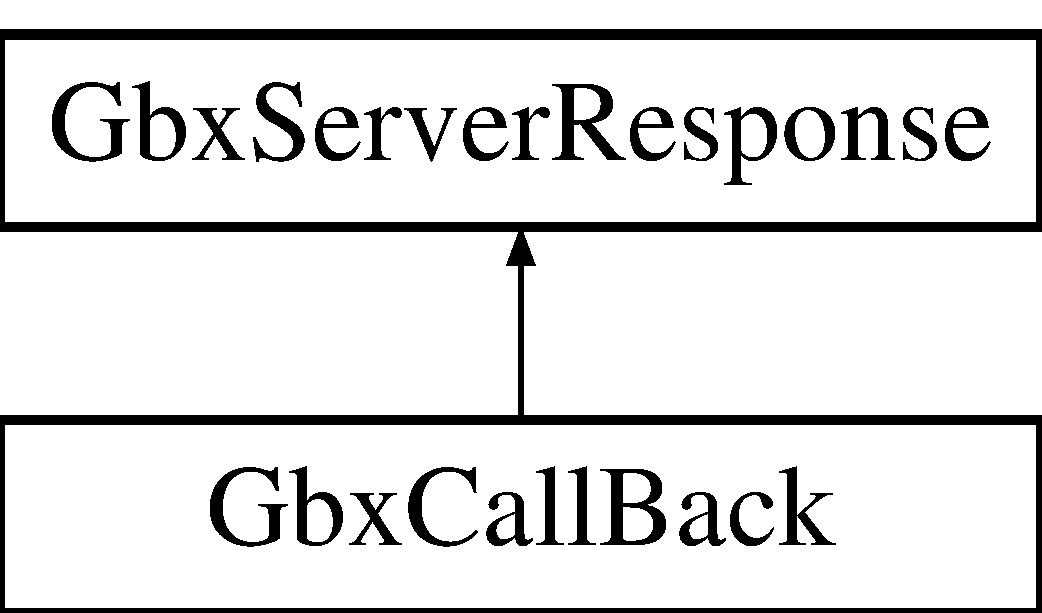
\includegraphics[height=2.000000cm]{classGbxCallBack}
\end{center}
\end{figure}
\subsection*{Public Member Functions}
\begin{DoxyCompactItemize}
\item 
char $\ast$ \hyperlink{classGbxCallBack_a434467d6000e1546e85f94885a816946}{Get\-Method\-Name} ()
\item 
void \hyperlink{classGbxCallBack_a78a993170ce1e3c5a35f02088e4f66a0}{Set\-Raw} (char $\ast$callback)
\begin{DoxyCompactList}\small\item\em Sets the raw message value. \end{DoxyCompactList}\item 
char $\ast$ \hyperlink{classGbxServerResponse_a3105f299a4f6a0d997f909415a467fd5}{Get\-Raw} ()
\begin{DoxyCompactList}\small\item\em Returns raw response (X\-M\-L). \end{DoxyCompactList}\item 
std\-::vector\\*
$<$ \hyperlink{classGbxResponseParameter}{Gbx\-Response\-Parameter} $>$ $\ast$ \hyperlink{classGbxServerResponse_ab791b8d9edb964b909d3c70753549668}{Get\-Parameters} ()
\begin{DoxyCompactList}\small\item\em Returns the extracted parameters. \end{DoxyCompactList}\end{DoxyCompactItemize}
\subsection*{Protected Member Functions}
\begin{DoxyCompactItemize}
\item 
\hyperlink{classGbxResponseParameter}{Gbx\-Response\-Parameter} \hyperlink{classGbxServerResponse_afa89ad0963df83f64934c9a54bb0dac6}{extract\-Param} (tinyxml2\-::\-X\-M\-L\-Element $\ast$param)
\begin{DoxyCompactList}\small\item\em Extracts parameters from the raw data (X\-M\-L). \end{DoxyCompactList}\end{DoxyCompactItemize}
\subsection*{Protected Attributes}
\begin{DoxyCompactItemize}
\item 
char $\ast$ \hyperlink{classGbxServerResponse_aeee1fc539a5881334926e5c6789581bd}{data}
\begin{DoxyCompactList}\small\item\em Raw response data. \end{DoxyCompactList}\item 
std\-::vector\\*
$<$ \hyperlink{classGbxResponseParameter}{Gbx\-Response\-Parameter} $>$ $\ast$ \hyperlink{classGbxServerResponse_ad6fef5319c4da9461f4cd0d72d8b5ee8}{parameters} = new std\-::vector$<$\hyperlink{classGbxResponseParameter}{Gbx\-Response\-Parameter}$>$()
\begin{DoxyCompactList}\small\item\em List of parameters. \end{DoxyCompactList}\end{DoxyCompactItemize}
\subsection*{Private Member Functions}
\begin{DoxyCompactItemize}
\item 
void \hyperlink{classGbxCallBack_a0a9b9db5ebdc8040058b542fb51283d7}{extract\-Parameters} ()
\begin{DoxyCompactList}\small\item\em Extracts parameters from the raw data (X\-M\-L). \end{DoxyCompactList}\end{DoxyCompactItemize}
\subsection*{Private Attributes}
\begin{DoxyCompactItemize}
\item 
char $\ast$ \hyperlink{classGbxCallBack_a767f111fc7851cf31b3bf86dfd816b85}{method\-Name}
\begin{DoxyCompactList}\small\item\em Method name. \end{DoxyCompactList}\end{DoxyCompactItemize}


\subsection{Detailed Description}
Call\-Back from server, de-\/\-X\-M\-L-\/fies the callback. 

\subsection{Member Function Documentation}
\hypertarget{classGbxServerResponse_afa89ad0963df83f64934c9a54bb0dac6}{\index{Gbx\-Call\-Back@{Gbx\-Call\-Back}!extract\-Param@{extract\-Param}}
\index{extract\-Param@{extract\-Param}!GbxCallBack@{Gbx\-Call\-Back}}
\subsubsection[{extract\-Param}]{\setlength{\rightskip}{0pt plus 5cm}{\bf Gbx\-Response\-Parameter} Gbx\-Server\-Response\-::extract\-Param (
\begin{DoxyParamCaption}
\item[{tinyxml2\-::\-X\-M\-L\-Element $\ast$}]{param}
\end{DoxyParamCaption}
)\hspace{0.3cm}{\ttfamily [protected]}, {\ttfamily [inherited]}}}\label{classGbxServerResponse_afa89ad0963df83f64934c9a54bb0dac6}


Extracts parameters from the raw data (X\-M\-L). 

\hypertarget{classGbxCallBack_a0a9b9db5ebdc8040058b542fb51283d7}{\index{Gbx\-Call\-Back@{Gbx\-Call\-Back}!extract\-Parameters@{extract\-Parameters}}
\index{extract\-Parameters@{extract\-Parameters}!GbxCallBack@{Gbx\-Call\-Back}}
\subsubsection[{extract\-Parameters}]{\setlength{\rightskip}{0pt plus 5cm}void Gbx\-Call\-Back\-::extract\-Parameters (
\begin{DoxyParamCaption}
{}
\end{DoxyParamCaption}
)\hspace{0.3cm}{\ttfamily [private]}}}\label{classGbxCallBack_a0a9b9db5ebdc8040058b542fb51283d7}


Extracts parameters from the raw data (X\-M\-L). 

\hypertarget{classGbxCallBack_a434467d6000e1546e85f94885a816946}{\index{Gbx\-Call\-Back@{Gbx\-Call\-Back}!Get\-Method\-Name@{Get\-Method\-Name}}
\index{Get\-Method\-Name@{Get\-Method\-Name}!GbxCallBack@{Gbx\-Call\-Back}}
\subsubsection[{Get\-Method\-Name}]{\setlength{\rightskip}{0pt plus 5cm}char $\ast$ Gbx\-Call\-Back\-::\-Get\-Method\-Name (
\begin{DoxyParamCaption}
{}
\end{DoxyParamCaption}
)}}\label{classGbxCallBack_a434467d6000e1546e85f94885a816946}
Returns the method name. \hypertarget{classGbxServerResponse_ab791b8d9edb964b909d3c70753549668}{\index{Gbx\-Call\-Back@{Gbx\-Call\-Back}!Get\-Parameters@{Get\-Parameters}}
\index{Get\-Parameters@{Get\-Parameters}!GbxCallBack@{Gbx\-Call\-Back}}
\subsubsection[{Get\-Parameters}]{\setlength{\rightskip}{0pt plus 5cm}std\-::vector$<$ {\bf Gbx\-Response\-Parameter} $>$ $\ast$ Gbx\-Server\-Response\-::\-Get\-Parameters (
\begin{DoxyParamCaption}
{}
\end{DoxyParamCaption}
)\hspace{0.3cm}{\ttfamily [inherited]}}}\label{classGbxServerResponse_ab791b8d9edb964b909d3c70753549668}


Returns the extracted parameters. 

\hypertarget{classGbxServerResponse_a3105f299a4f6a0d997f909415a467fd5}{\index{Gbx\-Call\-Back@{Gbx\-Call\-Back}!Get\-Raw@{Get\-Raw}}
\index{Get\-Raw@{Get\-Raw}!GbxCallBack@{Gbx\-Call\-Back}}
\subsubsection[{Get\-Raw}]{\setlength{\rightskip}{0pt plus 5cm}char $\ast$ Gbx\-Server\-Response\-::\-Get\-Raw (
\begin{DoxyParamCaption}
{}
\end{DoxyParamCaption}
)\hspace{0.3cm}{\ttfamily [inherited]}}}\label{classGbxServerResponse_a3105f299a4f6a0d997f909415a467fd5}


Returns raw response (X\-M\-L). 

\hypertarget{classGbxCallBack_a78a993170ce1e3c5a35f02088e4f66a0}{\index{Gbx\-Call\-Back@{Gbx\-Call\-Back}!Set\-Raw@{Set\-Raw}}
\index{Set\-Raw@{Set\-Raw}!GbxCallBack@{Gbx\-Call\-Back}}
\subsubsection[{Set\-Raw}]{\setlength{\rightskip}{0pt plus 5cm}void Gbx\-Call\-Back\-::\-Set\-Raw (
\begin{DoxyParamCaption}
\item[{char $\ast$}]{callback}
\end{DoxyParamCaption}
)}}\label{classGbxCallBack_a78a993170ce1e3c5a35f02088e4f66a0}


Sets the raw message value. 


\begin{DoxyParams}{Parameters}
{\em callback} & Raw callback from server (X\-M\-L). \\
\hline
\end{DoxyParams}


\subsection{Member Data Documentation}
\hypertarget{classGbxServerResponse_aeee1fc539a5881334926e5c6789581bd}{\index{Gbx\-Call\-Back@{Gbx\-Call\-Back}!data@{data}}
\index{data@{data}!GbxCallBack@{Gbx\-Call\-Back}}
\subsubsection[{data}]{\setlength{\rightskip}{0pt plus 5cm}char$\ast$ Gbx\-Server\-Response\-::data\hspace{0.3cm}{\ttfamily [protected]}, {\ttfamily [inherited]}}}\label{classGbxServerResponse_aeee1fc539a5881334926e5c6789581bd}


Raw response data. 

\hypertarget{classGbxCallBack_a767f111fc7851cf31b3bf86dfd816b85}{\index{Gbx\-Call\-Back@{Gbx\-Call\-Back}!method\-Name@{method\-Name}}
\index{method\-Name@{method\-Name}!GbxCallBack@{Gbx\-Call\-Back}}
\subsubsection[{method\-Name}]{\setlength{\rightskip}{0pt plus 5cm}char$\ast$ Gbx\-Call\-Back\-::method\-Name\hspace{0.3cm}{\ttfamily [private]}}}\label{classGbxCallBack_a767f111fc7851cf31b3bf86dfd816b85}


Method name. 

\hypertarget{classGbxServerResponse_ad6fef5319c4da9461f4cd0d72d8b5ee8}{\index{Gbx\-Call\-Back@{Gbx\-Call\-Back}!parameters@{parameters}}
\index{parameters@{parameters}!GbxCallBack@{Gbx\-Call\-Back}}
\subsubsection[{parameters}]{\setlength{\rightskip}{0pt plus 5cm}std\-::vector$<${\bf Gbx\-Response\-Parameter}$>$$\ast$ Gbx\-Server\-Response\-::parameters = new std\-::vector$<${\bf Gbx\-Response\-Parameter}$>$()\hspace{0.3cm}{\ttfamily [protected]}, {\ttfamily [inherited]}}}\label{classGbxServerResponse_ad6fef5319c4da9461f4cd0d72d8b5ee8}


List of parameters. 



The documentation for this class was generated from the following files\-:\begin{DoxyCompactItemize}
\item 
/home/travis/build/\-The\-Maximum/mania-\/pp/src/\-Gbx\-Remote/\-Call\-Back/\hyperlink{GbxCallBack_8h}{Gbx\-Call\-Back.\-h}\item 
/home/travis/build/\-The\-Maximum/mania-\/pp/src/\-Gbx\-Remote/\-Call\-Back/\hyperlink{GbxCallBack_8cpp}{Gbx\-Call\-Back.\-cpp}\end{DoxyCompactItemize}

\hypertarget{structGbxError}{\section{Gbx\-Error Struct Reference}
\label{structGbxError}\index{Gbx\-Error@{Gbx\-Error}}
}


Stores error details from the communication with the server.  




{\ttfamily \#include $<$Gbx\-Structs.\-h$>$}

\subsection*{Public Attributes}
\begin{DoxyCompactItemize}
\item 
int \hyperlink{structGbxError_ae5627cae63e837beaa75f798e47be50e}{number} = 0
\begin{DoxyCompactList}\small\item\em Number of the error (default\-: 0, no error). \end{DoxyCompactList}\item 
std\-::string \hyperlink{structGbxError_af52353692b5c160deac99c4285f01a5a}{message}
\begin{DoxyCompactList}\small\item\em Error message. \end{DoxyCompactList}\end{DoxyCompactItemize}


\subsection{Detailed Description}
Stores error details from the communication with the server. 

\subsection{Member Data Documentation}
\hypertarget{structGbxError_af52353692b5c160deac99c4285f01a5a}{\index{Gbx\-Error@{Gbx\-Error}!message@{message}}
\index{message@{message}!GbxError@{Gbx\-Error}}
\subsubsection[{message}]{\setlength{\rightskip}{0pt plus 5cm}std\-::string Gbx\-Error\-::message}}\label{structGbxError_af52353692b5c160deac99c4285f01a5a}


Error message. 

\hypertarget{structGbxError_ae5627cae63e837beaa75f798e47be50e}{\index{Gbx\-Error@{Gbx\-Error}!number@{number}}
\index{number@{number}!GbxError@{Gbx\-Error}}
\subsubsection[{number}]{\setlength{\rightskip}{0pt plus 5cm}int Gbx\-Error\-::number = 0}}\label{structGbxError_ae5627cae63e837beaa75f798e47be50e}


Number of the error (default\-: 0, no error). 



The documentation for this struct was generated from the following file\-:\begin{DoxyCompactItemize}
\item 
/home/travis/build/\-The\-Maximum/mania-\/pp/src/\-Gbx\-Remote/\hyperlink{GbxStructs_8h}{Gbx\-Structs.\-h}\end{DoxyCompactItemize}

\hypertarget{structGbxFirstResponse}{\section{Gbx\-First\-Response Struct Reference}
\label{structGbxFirstResponse}\index{Gbx\-First\-Response@{Gbx\-First\-Response}}
}


Response received on handshake.  




{\ttfamily \#include $<$Gbx\-Structs.\-h$>$}

\subsection*{Public Attributes}
\begin{DoxyCompactItemize}
\item 
short \hyperlink{structGbxFirstResponse_ad93a9c67024b28ecddb779457dd001f8}{size}
\begin{DoxyCompactList}\small\item\em Size in bytes of the protocol message (usually 11). \end{DoxyCompactList}\end{DoxyCompactItemize}


\subsection{Detailed Description}
Response received on handshake. 

\subsection{Member Data Documentation}
\hypertarget{structGbxFirstResponse_ad93a9c67024b28ecddb779457dd001f8}{\index{Gbx\-First\-Response@{Gbx\-First\-Response}!size@{size}}
\index{size@{size}!GbxFirstResponse@{Gbx\-First\-Response}}
\subsubsection[{size}]{\setlength{\rightskip}{0pt plus 5cm}short Gbx\-First\-Response\-::size}}\label{structGbxFirstResponse_ad93a9c67024b28ecddb779457dd001f8}


Size in bytes of the protocol message (usually 11). 



The documentation for this struct was generated from the following file\-:\begin{DoxyCompactItemize}
\item 
/home/travis/build/\-The\-Maximum/mania-\/pp/src/\-Gbx\-Remote/\hyperlink{GbxStructs_8h}{Gbx\-Structs.\-h}\end{DoxyCompactItemize}

\hypertarget{classGbxMessage}{\section{Gbx\-Message Class Reference}
\label{classGbxMessage}\index{Gbx\-Message@{Gbx\-Message}}
}


X\-M\-L-\/fies the message for communication with the server.  




{\ttfamily \#include $<$Gbx\-Message.\-h$>$}

\subsection*{Public Member Functions}
\begin{DoxyCompactItemize}
\item 
\hyperlink{classGbxMessage_ad4a5e5f75787e12229cf03aabc4ad930}{Gbx\-Message} (std\-::string \hyperlink{classGbxMessage_a10b6118916999db98f28e3f495eef6b4}{method}, \hyperlink{classGbxParameters}{Gbx\-Parameters} $\ast$parameters=N\-U\-L\-L)
\begin{DoxyCompactList}\small\item\em Builds X\-M\-L message. \end{DoxyCompactList}\item 
std\-::string \hyperlink{classGbxMessage_a53e00a162c293251bef476ad74d0134c}{Get\-Method} ()
\begin{DoxyCompactList}\small\item\em Returns the method name. \end{DoxyCompactList}\item 
std\-::string \hyperlink{classGbxMessage_ac81e16efce7da483a696d6653e18c9d8}{Get\-Xml} ()
\begin{DoxyCompactList}\small\item\em Returns the created X\-M\-L message. \end{DoxyCompactList}\end{DoxyCompactItemize}
\subsection*{Private Attributes}
\begin{DoxyCompactItemize}
\item 
std\-::string \hyperlink{classGbxMessage_a10b6118916999db98f28e3f495eef6b4}{method}
\begin{DoxyCompactList}\small\item\em Server method name. \end{DoxyCompactList}\item 
std\-::string \hyperlink{classGbxMessage_a6ea9adbeb3f1c104fa08fce0b1a4090d}{xml}
\begin{DoxyCompactList}\small\item\em Created X\-M\-L message. \end{DoxyCompactList}\end{DoxyCompactItemize}


\subsection{Detailed Description}
X\-M\-L-\/fies the message for communication with the server. 

\subsection{Constructor \& Destructor Documentation}
\hypertarget{classGbxMessage_ad4a5e5f75787e12229cf03aabc4ad930}{\index{Gbx\-Message@{Gbx\-Message}!Gbx\-Message@{Gbx\-Message}}
\index{Gbx\-Message@{Gbx\-Message}!GbxMessage@{Gbx\-Message}}
\subsubsection[{Gbx\-Message}]{\setlength{\rightskip}{0pt plus 5cm}Gbx\-Message\-::\-Gbx\-Message (
\begin{DoxyParamCaption}
\item[{std\-::string}]{method, }
\item[{{\bf Gbx\-Parameters} $\ast$}]{parameters = {\ttfamily NULL}}
\end{DoxyParamCaption}
)}}\label{classGbxMessage_ad4a5e5f75787e12229cf03aabc4ad930}


Builds X\-M\-L message. 


\begin{DoxyParams}{Parameters}
{\em method} & Server method name. \\
\hline
{\em params} & Params which belong to the method. \\
\hline
\end{DoxyParams}


\subsection{Member Function Documentation}
\hypertarget{classGbxMessage_a53e00a162c293251bef476ad74d0134c}{\index{Gbx\-Message@{Gbx\-Message}!Get\-Method@{Get\-Method}}
\index{Get\-Method@{Get\-Method}!GbxMessage@{Gbx\-Message}}
\subsubsection[{Get\-Method}]{\setlength{\rightskip}{0pt plus 5cm}std\-::string Gbx\-Message\-::\-Get\-Method (
\begin{DoxyParamCaption}
{}
\end{DoxyParamCaption}
)}}\label{classGbxMessage_a53e00a162c293251bef476ad74d0134c}


Returns the method name. 

\hypertarget{classGbxMessage_ac81e16efce7da483a696d6653e18c9d8}{\index{Gbx\-Message@{Gbx\-Message}!Get\-Xml@{Get\-Xml}}
\index{Get\-Xml@{Get\-Xml}!GbxMessage@{Gbx\-Message}}
\subsubsection[{Get\-Xml}]{\setlength{\rightskip}{0pt plus 5cm}std\-::string Gbx\-Message\-::\-Get\-Xml (
\begin{DoxyParamCaption}
{}
\end{DoxyParamCaption}
)}}\label{classGbxMessage_ac81e16efce7da483a696d6653e18c9d8}


Returns the created X\-M\-L message. 



\subsection{Member Data Documentation}
\hypertarget{classGbxMessage_a10b6118916999db98f28e3f495eef6b4}{\index{Gbx\-Message@{Gbx\-Message}!method@{method}}
\index{method@{method}!GbxMessage@{Gbx\-Message}}
\subsubsection[{method}]{\setlength{\rightskip}{0pt plus 5cm}std\-::string Gbx\-Message\-::method\hspace{0.3cm}{\ttfamily [private]}}}\label{classGbxMessage_a10b6118916999db98f28e3f495eef6b4}


Server method name. 

\hypertarget{classGbxMessage_a6ea9adbeb3f1c104fa08fce0b1a4090d}{\index{Gbx\-Message@{Gbx\-Message}!xml@{xml}}
\index{xml@{xml}!GbxMessage@{Gbx\-Message}}
\subsubsection[{xml}]{\setlength{\rightskip}{0pt plus 5cm}std\-::string Gbx\-Message\-::xml\hspace{0.3cm}{\ttfamily [private]}}}\label{classGbxMessage_a6ea9adbeb3f1c104fa08fce0b1a4090d}


Created X\-M\-L message. 



The documentation for this class was generated from the following files\-:\begin{DoxyCompactItemize}
\item 
/home/travis/build/\-The\-Maximum/mania-\/pp/src/\-Gbx\-Remote/\hyperlink{GbxMessage_8h}{Gbx\-Message.\-h}\item 
/home/travis/build/\-The\-Maximum/mania-\/pp/src/\-Gbx\-Remote/\hyperlink{GbxMessage_8cpp}{Gbx\-Message.\-cpp}\end{DoxyCompactItemize}

\hypertarget{structGbxParam}{\section{Gbx\-Param Struct Reference}
\label{structGbxParam}\index{Gbx\-Param@{Gbx\-Param}}
}


Pointer and type information of a parameter.  




{\ttfamily \#include $<$Gbx\-Parameters.\-h$>$}

\subsection*{Public Attributes}
\begin{DoxyCompactItemize}
\item 
void $\ast$ \hyperlink{structGbxParam_a19b53f8dacdd8937e1020775f8615495}{pointer}
\begin{DoxyCompactList}\small\item\em Pointer to the parameter. \end{DoxyCompactList}\item 
const std\-::type\-\_\-info $\ast$ \hyperlink{structGbxParam_afb3596a5ba95fda1e27a5c6b4ed517b5}{typeinfo}
\begin{DoxyCompactList}\small\item\em Type information of the parameter. \end{DoxyCompactList}\end{DoxyCompactItemize}


\subsection{Detailed Description}
Pointer and type information of a parameter. 

\subsection{Member Data Documentation}
\hypertarget{structGbxParam_a19b53f8dacdd8937e1020775f8615495}{\index{Gbx\-Param@{Gbx\-Param}!pointer@{pointer}}
\index{pointer@{pointer}!GbxParam@{Gbx\-Param}}
\subsubsection[{pointer}]{\setlength{\rightskip}{0pt plus 5cm}void$\ast$ Gbx\-Param\-::pointer}}\label{structGbxParam_a19b53f8dacdd8937e1020775f8615495}


Pointer to the parameter. 

\hypertarget{structGbxParam_afb3596a5ba95fda1e27a5c6b4ed517b5}{\index{Gbx\-Param@{Gbx\-Param}!typeinfo@{typeinfo}}
\index{typeinfo@{typeinfo}!GbxParam@{Gbx\-Param}}
\subsubsection[{typeinfo}]{\setlength{\rightskip}{0pt plus 5cm}const std\-::type\-\_\-info$\ast$ Gbx\-Param\-::typeinfo}}\label{structGbxParam_afb3596a5ba95fda1e27a5c6b4ed517b5}


Type information of the parameter. 



The documentation for this struct was generated from the following file\-:\begin{DoxyCompactItemize}
\item 
/home/travis/build/\-The\-Maximum/mania-\/pp/src/\-Gbx\-Remote/\-Parameters/\hyperlink{GbxParameters_8h}{Gbx\-Parameters.\-h}\end{DoxyCompactItemize}

\hypertarget{classGbxParameter}{\section{Gbx\-Parameter Class Reference}
\label{classGbxParameter}\index{Gbx\-Parameter@{Gbx\-Parameter}}
}


X\-M\-L-\/fies the parameter for communication with the server.  




{\ttfamily \#include $<$Gbx\-Parameter.\-h$>$}

\subsection*{Public Member Functions}
\begin{DoxyCompactItemize}
\item 
\hyperlink{classGbxParameter_a6cfd5c21c176ca6d9d2a1a3d9ad9953c}{Gbx\-Parameter} (\hyperlink{structGbxParam}{Gbx\-Param} param)
\begin{DoxyCompactList}\small\item\em Casts parameter to string and calls calculate\-Type. \end{DoxyCompactList}\item 
\hypertarget{classGbxParameter_a3c6800bca78c5bb4ed7de62cf552ee35}{std\-::string \hyperlink{classGbxParameter_a3c6800bca78c5bb4ed7de62cf552ee35}{Get\-Xml} ()}\label{classGbxParameter_a3c6800bca78c5bb4ed7de62cf552ee35}

\begin{DoxyCompactList}\small\item\em Returns xml-\/fied parameter. \end{DoxyCompactList}\end{DoxyCompactItemize}
\subsection*{Private Member Functions}
\begin{DoxyCompactItemize}
\item 
void \hyperlink{classGbxParameter_af708857623b85684ede2ae002e53a118}{determine\-Type} (const std\-::type\-\_\-info $\ast$param)
\begin{DoxyCompactList}\small\item\em Determines which X\-M\-L-\/\-R\-P\-C type the parameter has. \end{DoxyCompactList}\item 
void \hyperlink{classGbxParameter_a8e038bca99e1eb7339567fe1af79586c}{dereference\-Data} (void $\ast$param)
\begin{DoxyCompactList}\small\item\em Converts the void pointer into the type determined in determine\-Type. \end{DoxyCompactList}\end{DoxyCompactItemize}
\subsection*{Private Attributes}
\begin{DoxyCompactItemize}
\item 
\hypertarget{classGbxParameter_a6b64cfaae4d5b3b498fb2cdd3d28f824}{std\-::string \hyperlink{classGbxParameter_a6b64cfaae4d5b3b498fb2cdd3d28f824}{data}}\label{classGbxParameter_a6b64cfaae4d5b3b498fb2cdd3d28f824}

\begin{DoxyCompactList}\small\item\em Stringified parameter. \end{DoxyCompactList}\item 
\hypertarget{classGbxParameter_a19d4cab065cb0440c675e97babf45d02}{std\-::string \hyperlink{classGbxParameter_a19d4cab065cb0440c675e97babf45d02}{type}}\label{classGbxParameter_a19d4cab065cb0440c675e97babf45d02}

\begin{DoxyCompactList}\small\item\em Stringified parameter type for X\-M\-L. \end{DoxyCompactList}\item 
\hypertarget{classGbxParameter_ad5182c3df0c77e011c61e00e182f8a49}{std\-::string \hyperlink{classGbxParameter_ad5182c3df0c77e011c61e00e182f8a49}{xml\-Type}}\label{classGbxParameter_ad5182c3df0c77e011c61e00e182f8a49}

\begin{DoxyCompactList}\small\item\em Stringified parameter type for X\-M\-L. \end{DoxyCompactList}\end{DoxyCompactItemize}


\subsection{Detailed Description}
X\-M\-L-\/fies the parameter for communication with the server. 

\subsection{Constructor \& Destructor Documentation}
\hypertarget{classGbxParameter_a6cfd5c21c176ca6d9d2a1a3d9ad9953c}{\index{Gbx\-Parameter@{Gbx\-Parameter}!Gbx\-Parameter@{Gbx\-Parameter}}
\index{Gbx\-Parameter@{Gbx\-Parameter}!GbxParameter@{Gbx\-Parameter}}
\subsubsection[{Gbx\-Parameter}]{\setlength{\rightskip}{0pt plus 5cm}Gbx\-Parameter\-::\-Gbx\-Parameter (
\begin{DoxyParamCaption}
\item[{{\bf Gbx\-Param}}]{param}
\end{DoxyParamCaption}
)}}\label{classGbxParameter_a6cfd5c21c176ca6d9d2a1a3d9ad9953c}


Casts parameter to string and calls calculate\-Type. 


\begin{DoxyParams}{Parameters}
{\em param} & Parameter to be xml-\/fied. \\
\hline
\end{DoxyParams}


\subsection{Member Function Documentation}
\hypertarget{classGbxParameter_a8e038bca99e1eb7339567fe1af79586c}{\index{Gbx\-Parameter@{Gbx\-Parameter}!dereference\-Data@{dereference\-Data}}
\index{dereference\-Data@{dereference\-Data}!GbxParameter@{Gbx\-Parameter}}
\subsubsection[{dereference\-Data}]{\setlength{\rightskip}{0pt plus 5cm}void Gbx\-Parameter\-::dereference\-Data (
\begin{DoxyParamCaption}
\item[{void $\ast$}]{param}
\end{DoxyParamCaption}
)\hspace{0.3cm}{\ttfamily [private]}}}\label{classGbxParameter_a8e038bca99e1eb7339567fe1af79586c}


Converts the void pointer into the type determined in determine\-Type. 


\begin{DoxyParams}{Parameters}
{\em param} & Void pointer to parameter. \\
\hline
\end{DoxyParams}
\hypertarget{classGbxParameter_af708857623b85684ede2ae002e53a118}{\index{Gbx\-Parameter@{Gbx\-Parameter}!determine\-Type@{determine\-Type}}
\index{determine\-Type@{determine\-Type}!GbxParameter@{Gbx\-Parameter}}
\subsubsection[{determine\-Type}]{\setlength{\rightskip}{0pt plus 5cm}void Gbx\-Parameter\-::determine\-Type (
\begin{DoxyParamCaption}
\item[{const std\-::type\-\_\-info $\ast$}]{param}
\end{DoxyParamCaption}
)\hspace{0.3cm}{\ttfamily [private]}}}\label{classGbxParameter_af708857623b85684ede2ae002e53a118}


Determines which X\-M\-L-\/\-R\-P\-C type the parameter has. 


\begin{DoxyParams}{Parameters}
{\em param} & Type information about the parameter. \\
\hline
\end{DoxyParams}


The documentation for this class was generated from the following files\-:\begin{DoxyCompactItemize}
\item 
/home/travis/build/\-The\-Maximum/mania-\/pp/src/\-Gbx\-Remote/\-Parameters/Gbx\-Parameter.\-h\item 
/home/travis/build/\-The\-Maximum/mania-\/pp/src/\-Gbx\-Remote/\-Parameters/Gbx\-Parameter.\-cpp\end{DoxyCompactItemize}

\hypertarget{classGbxParameters}{\section{Gbx\-Parameters Class Reference}
\label{classGbxParameters}\index{Gbx\-Parameters@{Gbx\-Parameters}}
}


List of parameters.  




{\ttfamily \#include $<$Gbx\-Parameters.\-h$>$}

\subsection*{Public Member Functions}
\begin{DoxyCompactItemize}
\item 
{\footnotesize template$<$typename T $>$ }\\void \hyperlink{classGbxParameters_a2cf83794717cf9fdc13e5ff12e259f04}{Put} (T $\ast$pointer)
\begin{DoxyCompactList}\small\item\em Add parameter to the list. \end{DoxyCompactList}\item 
\hypertarget{classGbxParameters_a09302bc40359205cd294b8bcf2ab1c2e}{std\-::vector$<$ \hyperlink{structGbxParam}{Gbx\-Param} $>$ \hyperlink{classGbxParameters_a09302bc40359205cd294b8bcf2ab1c2e}{Get\-Parameters} ()}\label{classGbxParameters_a09302bc40359205cd294b8bcf2ab1c2e}

\begin{DoxyCompactList}\small\item\em Return the current list of parameters. \end{DoxyCompactList}\end{DoxyCompactItemize}
\subsection*{Private Attributes}
\begin{DoxyCompactItemize}
\item 
\hypertarget{classGbxParameters_aeabcb21396d3198d718c94de23595750}{std\-::vector$<$ \hyperlink{structGbxParam}{Gbx\-Param} $>$ \hyperlink{classGbxParameters_aeabcb21396d3198d718c94de23595750}{parameters} = std\-::vector$<$\hyperlink{structGbxParam}{Gbx\-Param}$>$()}\label{classGbxParameters_aeabcb21396d3198d718c94de23595750}

\begin{DoxyCompactList}\small\item\em List of parameters. \end{DoxyCompactList}\end{DoxyCompactItemize}


\subsection{Detailed Description}
List of parameters. 

\subsection{Member Function Documentation}
\hypertarget{classGbxParameters_a2cf83794717cf9fdc13e5ff12e259f04}{\index{Gbx\-Parameters@{Gbx\-Parameters}!Put@{Put}}
\index{Put@{Put}!GbxParameters@{Gbx\-Parameters}}
\subsubsection[{Put}]{\setlength{\rightskip}{0pt plus 5cm}template$<$typename T $>$ void Gbx\-Parameters\-::\-Put (
\begin{DoxyParamCaption}
\item[{T $\ast$}]{pointer}
\end{DoxyParamCaption}
)\hspace{0.3cm}{\ttfamily [inline]}}}\label{classGbxParameters_a2cf83794717cf9fdc13e5ff12e259f04}


Add parameter to the list. 


\begin{DoxyParams}{Parameters}
{\em pointer} & Pointer to the parameter. \\
\hline
\end{DoxyParams}


The documentation for this class was generated from the following file\-:\begin{DoxyCompactItemize}
\item 
/home/travis/build/\-The\-Maximum/mania-\/pp/src/\-Gbx\-Remote/\-Parameters/Gbx\-Parameters.\-h\end{DoxyCompactItemize}

\hypertarget{structGbxQueryResponse}{\section{Gbx\-Query\-Response Struct Reference}
\label{structGbxQueryResponse}\index{Gbx\-Query\-Response@{Gbx\-Query\-Response}}
}


Response received after a query is sent.  




{\ttfamily \#include $<$Gbx\-Structs.\-h$>$}

\subsection*{Public Attributes}
\begin{DoxyCompactItemize}
\item 
short \hyperlink{structGbxQueryResponse_ab7d7e30d6beb443cdae8cbf95e4c89f3}{size}
\begin{DoxyCompactList}\small\item\em Size in bytes of the query response. \end{DoxyCompactList}\item 
long \hyperlink{structGbxQueryResponse_ad37f7d084a89880263a2a36287427af3}{handle}
\begin{DoxyCompactList}\small\item\em Handle identifier of response message. \end{DoxyCompactList}\end{DoxyCompactItemize}


\subsection{Detailed Description}
Response received after a query is sent. 

\subsection{Member Data Documentation}
\hypertarget{structGbxQueryResponse_ad37f7d084a89880263a2a36287427af3}{\index{Gbx\-Query\-Response@{Gbx\-Query\-Response}!handle@{handle}}
\index{handle@{handle}!GbxQueryResponse@{Gbx\-Query\-Response}}
\subsubsection[{handle}]{\setlength{\rightskip}{0pt plus 5cm}long Gbx\-Query\-Response\-::handle}}\label{structGbxQueryResponse_ad37f7d084a89880263a2a36287427af3}


Handle identifier of response message. 

\hypertarget{structGbxQueryResponse_ab7d7e30d6beb443cdae8cbf95e4c89f3}{\index{Gbx\-Query\-Response@{Gbx\-Query\-Response}!size@{size}}
\index{size@{size}!GbxQueryResponse@{Gbx\-Query\-Response}}
\subsubsection[{size}]{\setlength{\rightskip}{0pt plus 5cm}short Gbx\-Query\-Response\-::size}}\label{structGbxQueryResponse_ab7d7e30d6beb443cdae8cbf95e4c89f3}


Size in bytes of the query response. 



The documentation for this struct was generated from the following file\-:\begin{DoxyCompactItemize}
\item 
/home/travis/build/\-The\-Maximum/mania-\/pp/src/\-Gbx\-Remote/\hyperlink{GbxStructs_8h}{Gbx\-Structs.\-h}\end{DoxyCompactItemize}

\hypertarget{classGbxRemote}{\section{Gbx\-Remote Class Reference}
\label{classGbxRemote}\index{Gbx\-Remote@{Gbx\-Remote}}
}


Handles communication with the Mania\-Planet server.  




{\ttfamily \#include $<$Gbx\-Remote.\-h$>$}

\subsection*{Public Member Functions}
\begin{DoxyCompactItemize}
\item 
\hyperlink{classGbxRemote_a9ac65a51eb6f9127337b4f99841cfe2d}{$\sim$\-Gbx\-Remote} ()
\item 
bool \hyperlink{classGbxRemote_a24d9d0df923ed85010f53dcb43c2b977}{Init} (int port)
\begin{DoxyCompactList}\small\item\em Initializes connection with the local server. \end{DoxyCompactList}\item 
bool \hyperlink{classGbxRemote_aa9a57e73f2f5ebbde90484503bd0d16d}{Init\-With\-Ip} (std\-::string address, int port)
\begin{DoxyCompactList}\small\item\em Initializes connection with the server. \end{DoxyCompactList}\item 
\hypertarget{classGbxRemote_a6fa8ca2d48aae84884cab98a0adf4360}{void \hyperlink{classGbxRemote_a6fa8ca2d48aae84884cab98a0adf4360}{Terminate} ()}\label{classGbxRemote_a6fa8ca2d48aae84884cab98a0adf4360}

\begin{DoxyCompactList}\small\item\em Closes the connection with the server. \end{DoxyCompactList}\item 
bool \hyperlink{classGbxRemote_a8ecc0e0625a8dca310cebd78bd2b3c7e}{Query} (\hyperlink{classGbxMessage}{Gbx\-Message} query)
\begin{DoxyCompactList}\small\item\em Sends a \hyperlink{classGbxMessage}{Gbx\-Message} to the server. \end{DoxyCompactList}\item 
bool \hyperlink{classGbxRemote_ac595861af2f4d7349ce3841f0758507d}{Read\-Call\-Backs} ()
\begin{DoxyCompactList}\small\item\em Read callbacks from the server. \end{DoxyCompactList}\item 
void \hyperlink{classGbxRemote_a5bd6e1dc2118f7e369e72592b3c9322a}{Handle\-Call\-Back} (std\-::string data)
\begin{DoxyCompactList}\small\item\em Handles callbacks (de-\/\-X\-M\-L-\/fies them). \end{DoxyCompactList}\item 
\hypertarget{classGbxRemote_a1ae6ff7eddcccdeda59af2316d053aae}{std\-::vector$<$ \hyperlink{classGbxCallBack}{Gbx\-Call\-Back} $>$ \hyperlink{classGbxRemote_a1ae6ff7eddcccdeda59af2316d053aae}{Get\-C\-B\-Responses} ()}\label{classGbxRemote_a1ae6ff7eddcccdeda59af2316d053aae}

\begin{DoxyCompactList}\small\item\em Returns the callbacks that have been received since last call. \end{DoxyCompactList}\item 
\hypertarget{classGbxRemote_a81ba62f042948610a3cf720316e22076}{void \hyperlink{classGbxRemote_a81ba62f042948610a3cf720316e22076}{Reset\-C\-B\-Responses} ()}\label{classGbxRemote_a81ba62f042948610a3cf720316e22076}

\begin{DoxyCompactList}\small\item\em Resets list of current callbacks. \end{DoxyCompactList}\item 
\hypertarget{classGbxRemote_adac67444e391ffcc1dfda8f087eaef0b}{\hyperlink{classGbxResponse}{Gbx\-Response} $\ast$ \hyperlink{classGbxRemote_adac67444e391ffcc1dfda8f087eaef0b}{Get\-Response} ()}\label{classGbxRemote_adac67444e391ffcc1dfda8f087eaef0b}

\begin{DoxyCompactList}\small\item\em Returns the response from the server. \end{DoxyCompactList}\item 
\hyperlink{structGbxError}{Gbx\-Error} \hyperlink{classGbxRemote_aa3f6e467372a23c3a53510d5488bea8a}{Get\-Current\-Error} ()
\begin{DoxyCompactList}\small\item\em Returns the current server error. \end{DoxyCompactList}\item 
\hypertarget{classGbxRemote_ae6e15060920a31482fd14045cfd42803}{int \hyperlink{classGbxRemote_ae6e15060920a31482fd14045cfd42803}{Get\-Protocol} ()}\label{classGbxRemote_ae6e15060920a31482fd14045cfd42803}

\begin{DoxyCompactList}\small\item\em Returns the current version number of the server protocol (1 or 2). \end{DoxyCompactList}\item 
\hypertarget{classGbxRemote_a6351f71fe649bff2aabfbd9b7c89e3f5}{std\-::string \hyperlink{classGbxRemote_a6351f71fe649bff2aabfbd9b7c89e3f5}{Get\-Api\-Version} ()}\label{classGbxRemote_a6351f71fe649bff2aabfbd9b7c89e3f5}

\begin{DoxyCompactList}\small\item\em Returns the set A\-P\-I version. \end{DoxyCompactList}\end{DoxyCompactItemize}
\subsection*{Private Attributes}
\begin{DoxyCompactItemize}
\item 
\hypertarget{classGbxRemote_a56662ea222345c645ae897e056b5c8c8}{bool \hyperlink{classGbxRemote_a56662ea222345c645ae897e056b5c8c8}{connected} = false}\label{classGbxRemote_a56662ea222345c645ae897e056b5c8c8}

\begin{DoxyCompactList}\small\item\em Is the client connected with the server? \end{DoxyCompactList}\item 
\hypertarget{classGbxRemote_a5ee5c7087085cb6cb2e7bc6135ff0646}{int \hyperlink{classGbxRemote_a5ee5c7087085cb6cb2e7bc6135ff0646}{protocol} = 0}\label{classGbxRemote_a5ee5c7087085cb6cb2e7bc6135ff0646}

\begin{DoxyCompactList}\small\item\em Protocol version (0 = uninitialized, 1 or 2 = version). \end{DoxyCompactList}\item 
\hypertarget{classGbxRemote_a81d3c0c70ab7f5e585840e9978ee900e}{std\-::string \hyperlink{classGbxRemote_a81d3c0c70ab7f5e585840e9978ee900e}{api\-Version}}\label{classGbxRemote_a81d3c0c70ab7f5e585840e9978ee900e}

\begin{DoxyCompactList}\small\item\em Server A\-P\-I version. \end{DoxyCompactList}\item 
\hypertarget{classGbxRemote_a0b0b212b945da4266fb645affdac81cb}{\hyperlink{classTcpClient}{Tcp\-Client} \hyperlink{classGbxRemote_a0b0b212b945da4266fb645affdac81cb}{server}}\label{classGbxRemote_a0b0b212b945da4266fb645affdac81cb}

\begin{DoxyCompactList}\small\item\em Socket connection with the server. \end{DoxyCompactList}\item 
\hypertarget{classGbxRemote_a5c310edc409e31aa12c0c0664b0fd238}{\hyperlink{structGbxError}{Gbx\-Error} \hyperlink{classGbxRemote_a5c310edc409e31aa12c0c0664b0fd238}{current\-Error} = \hyperlink{structGbxError}{Gbx\-Error}()}\label{classGbxRemote_a5c310edc409e31aa12c0c0664b0fd238}

\begin{DoxyCompactList}\small\item\em Current server error. \end{DoxyCompactList}\item 
\hypertarget{classGbxRemote_a3a3a0af1a692a801a33baa292b877dc2}{\hyperlink{classGbxResponse}{Gbx\-Response} $\ast$ \hyperlink{classGbxRemote_a3a3a0af1a692a801a33baa292b877dc2}{current\-Response} = new \hyperlink{classGbxResponse}{Gbx\-Response}}\label{classGbxRemote_a3a3a0af1a692a801a33baa292b877dc2}

\begin{DoxyCompactList}\small\item\em Current server response. \end{DoxyCompactList}\item 
\hypertarget{classGbxRemote_a08d047d7e0d4b746fc036c1aa02f0d17}{std\-::vector$<$ \hyperlink{classGbxCallBack}{Gbx\-Call\-Back} $>$ \hyperlink{classGbxRemote_a08d047d7e0d4b746fc036c1aa02f0d17}{current\-Call\-Backs} = std\-::vector$<$\hyperlink{classGbxCallBack}{Gbx\-Call\-Back}$>$()}\label{classGbxRemote_a08d047d7e0d4b746fc036c1aa02f0d17}

\begin{DoxyCompactList}\small\item\em List of currently received callbacks. \end{DoxyCompactList}\end{DoxyCompactItemize}


\subsection{Detailed Description}
Handles communication with the Mania\-Planet server. 

\begin{DoxyRefDesc}{Todo}
\item[\hyperlink{todo__todo000002}{Todo}]Make it possible to set an A\-P\-I version without upsetting Tiny\-X\-M\-L2. \end{DoxyRefDesc}


\subsection{Constructor \& Destructor Documentation}
\hypertarget{classGbxRemote_a9ac65a51eb6f9127337b4f99841cfe2d}{\index{Gbx\-Remote@{Gbx\-Remote}!$\sim$\-Gbx\-Remote@{$\sim$\-Gbx\-Remote}}
\index{$\sim$\-Gbx\-Remote@{$\sim$\-Gbx\-Remote}!GbxRemote@{Gbx\-Remote}}
\subsubsection[{$\sim$\-Gbx\-Remote}]{\setlength{\rightskip}{0pt plus 5cm}Gbx\-Remote\-::$\sim$\-Gbx\-Remote (
\begin{DoxyParamCaption}
{}
\end{DoxyParamCaption}
)}}\label{classGbxRemote_a9ac65a51eb6f9127337b4f99841cfe2d}
Deletes and nullifies the current\-Error and current\-Response. 

\subsection{Member Function Documentation}
\hypertarget{classGbxRemote_aa3f6e467372a23c3a53510d5488bea8a}{\index{Gbx\-Remote@{Gbx\-Remote}!Get\-Current\-Error@{Get\-Current\-Error}}
\index{Get\-Current\-Error@{Get\-Current\-Error}!GbxRemote@{Gbx\-Remote}}
\subsubsection[{Get\-Current\-Error}]{\setlength{\rightskip}{0pt plus 5cm}{\bf Gbx\-Error} Gbx\-Remote\-::\-Get\-Current\-Error (
\begin{DoxyParamCaption}
{}
\end{DoxyParamCaption}
)}}\label{classGbxRemote_aa3f6e467372a23c3a53510d5488bea8a}


Returns the current server error. 

Returns empty \hyperlink{structGbxError}{Gbx\-Error} when there currently is no error. \hypertarget{classGbxRemote_a5bd6e1dc2118f7e369e72592b3c9322a}{\index{Gbx\-Remote@{Gbx\-Remote}!Handle\-Call\-Back@{Handle\-Call\-Back}}
\index{Handle\-Call\-Back@{Handle\-Call\-Back}!GbxRemote@{Gbx\-Remote}}
\subsubsection[{Handle\-Call\-Back}]{\setlength{\rightskip}{0pt plus 5cm}void Gbx\-Remote\-::\-Handle\-Call\-Back (
\begin{DoxyParamCaption}
\item[{std\-::string}]{data}
\end{DoxyParamCaption}
)}}\label{classGbxRemote_a5bd6e1dc2118f7e369e72592b3c9322a}


Handles callbacks (de-\/\-X\-M\-L-\/fies them). 


\begin{DoxyParams}{Parameters}
{\em data} & Raw response from the server. \\
\hline
\end{DoxyParams}
\hypertarget{classGbxRemote_a24d9d0df923ed85010f53dcb43c2b977}{\index{Gbx\-Remote@{Gbx\-Remote}!Init@{Init}}
\index{Init@{Init}!GbxRemote@{Gbx\-Remote}}
\subsubsection[{Init}]{\setlength{\rightskip}{0pt plus 5cm}bool Gbx\-Remote\-::\-Init (
\begin{DoxyParamCaption}
\item[{int}]{port}
\end{DoxyParamCaption}
)}}\label{classGbxRemote_a24d9d0df923ed85010f53dcb43c2b977}


Initializes connection with the local server. 


\begin{DoxyParams}{Parameters}
{\em port} & X\-M\-L-\/\-R\-P\-C port of the server. \\
\hline
\end{DoxyParams}
\hypertarget{classGbxRemote_aa9a57e73f2f5ebbde90484503bd0d16d}{\index{Gbx\-Remote@{Gbx\-Remote}!Init\-With\-Ip@{Init\-With\-Ip}}
\index{Init\-With\-Ip@{Init\-With\-Ip}!GbxRemote@{Gbx\-Remote}}
\subsubsection[{Init\-With\-Ip}]{\setlength{\rightskip}{0pt plus 5cm}bool Gbx\-Remote\-::\-Init\-With\-Ip (
\begin{DoxyParamCaption}
\item[{std\-::string}]{address, }
\item[{int}]{port}
\end{DoxyParamCaption}
)}}\label{classGbxRemote_aa9a57e73f2f5ebbde90484503bd0d16d}


Initializes connection with the server. 


\begin{DoxyParams}{Parameters}
{\em address} & Address of the server. \\
\hline
{\em port} & X\-M\-L-\/\-R\-P\-C port of the server. \\
\hline
\end{DoxyParams}
\hypertarget{classGbxRemote_a8ecc0e0625a8dca310cebd78bd2b3c7e}{\index{Gbx\-Remote@{Gbx\-Remote}!Query@{Query}}
\index{Query@{Query}!GbxRemote@{Gbx\-Remote}}
\subsubsection[{Query}]{\setlength{\rightskip}{0pt plus 5cm}bool Gbx\-Remote\-::\-Query (
\begin{DoxyParamCaption}
\item[{{\bf Gbx\-Message}}]{query}
\end{DoxyParamCaption}
)}}\label{classGbxRemote_a8ecc0e0625a8dca310cebd78bd2b3c7e}


Sends a \hyperlink{classGbxMessage}{Gbx\-Message} to the server. 

Returns whether the query was successfully sent.


\begin{DoxyParams}{Parameters}
{\em query} & Query to be send. \\
\hline
\end{DoxyParams}
\hypertarget{classGbxRemote_ac595861af2f4d7349ce3841f0758507d}{\index{Gbx\-Remote@{Gbx\-Remote}!Read\-Call\-Backs@{Read\-Call\-Backs}}
\index{Read\-Call\-Backs@{Read\-Call\-Backs}!GbxRemote@{Gbx\-Remote}}
\subsubsection[{Read\-Call\-Backs}]{\setlength{\rightskip}{0pt plus 5cm}bool Gbx\-Remote\-::\-Read\-Call\-Backs (
\begin{DoxyParamCaption}
{}
\end{DoxyParamCaption}
)}}\label{classGbxRemote_ac595861af2f4d7349ce3841f0758507d}


Read callbacks from the server. 

Returns whether it found a callback. 

The documentation for this class was generated from the following files\-:\begin{DoxyCompactItemize}
\item 
/home/travis/build/\-The\-Maximum/mania-\/pp/src/\-Gbx\-Remote/Gbx\-Remote.\-h\item 
/home/travis/build/\-The\-Maximum/mania-\/pp/src/\-Gbx\-Remote/Gbx\-Remote.\-cpp\end{DoxyCompactItemize}

\hypertarget{classGbxResponse}{\section{Gbx\-Response Class Reference}
\label{classGbxResponse}\index{Gbx\-Response@{Gbx\-Response}}
}


Response from server, de-\/\-X\-M\-L-\/fies the response.  




{\ttfamily \#include $<$Gbx\-Response.\-h$>$}

\subsection*{Public Member Functions}
\begin{DoxyCompactItemize}
\item 
\hyperlink{classGbxResponse_ae29114aa0014ca50f3be6455bda1be47}{Gbx\-Response} ()
\begin{DoxyCompactList}\small\item\em Empty constructor. \end{DoxyCompactList}\item 
\hyperlink{classGbxResponse_a27e6c9c3452f2a0c90a33177af84236b}{$\sim$\-Gbx\-Response} ()
\item 
void \hyperlink{classGbxResponse_aadd25f4d4c454bb837af9b442742ff70}{Set\-Raw} (char $\ast$response)
\begin{DoxyCompactList}\small\item\em Sets the raw message value. \end{DoxyCompactList}\item 
char $\ast$ \hyperlink{classGbxResponse_a3311b30d7e04c2a14eb5f675ad6e37cd}{Get\-Raw} ()
\begin{DoxyCompactList}\small\item\em Returns raw response (X\-M\-L). \end{DoxyCompactList}\item 
std\-::vector\\*
$<$ \hyperlink{classGbxResponseParameter}{Gbx\-Response\-Parameter} $>$ $\ast$ \hyperlink{classGbxResponse_a9323a43f94e895422a7ee29a1eb80cc3}{Get\-Parameters} ()
\begin{DoxyCompactList}\small\item\em Returns the extracted parameters. \end{DoxyCompactList}\end{DoxyCompactItemize}
\subsection*{Private Member Functions}
\begin{DoxyCompactItemize}
\item 
void \hyperlink{classGbxResponse_a3cd4d6c5458fcd5359b8f5d9921a2a9b}{extract\-Parameters} ()
\begin{DoxyCompactList}\small\item\em Extracts parameters from the raw data (X\-M\-L). \end{DoxyCompactList}\item 
\hyperlink{classGbxResponseParameter}{Gbx\-Response\-Parameter} \hyperlink{classGbxResponse_af8501950f3b82ce74924f3bda746871b}{extract\-Param} (tinyxml2\-::\-X\-M\-L\-Element $\ast$param)
\begin{DoxyCompactList}\small\item\em Extracts parameters from the raw data (X\-M\-L). \end{DoxyCompactList}\end{DoxyCompactItemize}
\subsection*{Private Attributes}
\begin{DoxyCompactItemize}
\item 
char $\ast$ \hyperlink{classGbxResponse_aee1c7b03d870c87883bd97740afd7675}{data}
\begin{DoxyCompactList}\small\item\em Raw response data. \end{DoxyCompactList}\item 
std\-::vector\\*
$<$ \hyperlink{classGbxResponseParameter}{Gbx\-Response\-Parameter} $>$ $\ast$ \hyperlink{classGbxResponse_afcbec4555fa682d9d1360ecff829d0f2}{parameters} = new std\-::vector$<$\hyperlink{classGbxResponseParameter}{Gbx\-Response\-Parameter}$>$()
\begin{DoxyCompactList}\small\item\em List of parameters. \end{DoxyCompactList}\end{DoxyCompactItemize}


\subsection{Detailed Description}
Response from server, de-\/\-X\-M\-L-\/fies the response. 

\subsection{Constructor \& Destructor Documentation}
\hypertarget{classGbxResponse_ae29114aa0014ca50f3be6455bda1be47}{\index{Gbx\-Response@{Gbx\-Response}!Gbx\-Response@{Gbx\-Response}}
\index{Gbx\-Response@{Gbx\-Response}!GbxResponse@{Gbx\-Response}}
\subsubsection[{Gbx\-Response}]{\setlength{\rightskip}{0pt plus 5cm}Gbx\-Response\-::\-Gbx\-Response (
\begin{DoxyParamCaption}
{}
\end{DoxyParamCaption}
)}}\label{classGbxResponse_ae29114aa0014ca50f3be6455bda1be47}


Empty constructor. 

\hypertarget{classGbxResponse_a27e6c9c3452f2a0c90a33177af84236b}{\index{Gbx\-Response@{Gbx\-Response}!$\sim$\-Gbx\-Response@{$\sim$\-Gbx\-Response}}
\index{$\sim$\-Gbx\-Response@{$\sim$\-Gbx\-Response}!GbxResponse@{Gbx\-Response}}
\subsubsection[{$\sim$\-Gbx\-Response}]{\setlength{\rightskip}{0pt plus 5cm}Gbx\-Response\-::$\sim$\-Gbx\-Response (
\begin{DoxyParamCaption}
{}
\end{DoxyParamCaption}
)}}\label{classGbxResponse_a27e6c9c3452f2a0c90a33177af84236b}
Delets and nullifies the parameters. 

\subsection{Member Function Documentation}
\hypertarget{classGbxResponse_af8501950f3b82ce74924f3bda746871b}{\index{Gbx\-Response@{Gbx\-Response}!extract\-Param@{extract\-Param}}
\index{extract\-Param@{extract\-Param}!GbxResponse@{Gbx\-Response}}
\subsubsection[{extract\-Param}]{\setlength{\rightskip}{0pt plus 5cm}{\bf Gbx\-Response\-Parameter} Gbx\-Response\-::extract\-Param (
\begin{DoxyParamCaption}
\item[{tinyxml2\-::\-X\-M\-L\-Element $\ast$}]{param}
\end{DoxyParamCaption}
)\hspace{0.3cm}{\ttfamily [private]}}}\label{classGbxResponse_af8501950f3b82ce74924f3bda746871b}


Extracts parameters from the raw data (X\-M\-L). 

\hypertarget{classGbxResponse_a3cd4d6c5458fcd5359b8f5d9921a2a9b}{\index{Gbx\-Response@{Gbx\-Response}!extract\-Parameters@{extract\-Parameters}}
\index{extract\-Parameters@{extract\-Parameters}!GbxResponse@{Gbx\-Response}}
\subsubsection[{extract\-Parameters}]{\setlength{\rightskip}{0pt plus 5cm}void Gbx\-Response\-::extract\-Parameters (
\begin{DoxyParamCaption}
{}
\end{DoxyParamCaption}
)\hspace{0.3cm}{\ttfamily [private]}}}\label{classGbxResponse_a3cd4d6c5458fcd5359b8f5d9921a2a9b}


Extracts parameters from the raw data (X\-M\-L). 

\begin{DoxyRefDesc}{Todo}
\item[\hyperlink{todo__todo000001}{Todo}]Add support for structs. \end{DoxyRefDesc}
\hypertarget{classGbxResponse_a9323a43f94e895422a7ee29a1eb80cc3}{\index{Gbx\-Response@{Gbx\-Response}!Get\-Parameters@{Get\-Parameters}}
\index{Get\-Parameters@{Get\-Parameters}!GbxResponse@{Gbx\-Response}}
\subsubsection[{Get\-Parameters}]{\setlength{\rightskip}{0pt plus 5cm}std\-::vector$<$ {\bf Gbx\-Response\-Parameter} $>$ $\ast$ Gbx\-Response\-::\-Get\-Parameters (
\begin{DoxyParamCaption}
{}
\end{DoxyParamCaption}
)}}\label{classGbxResponse_a9323a43f94e895422a7ee29a1eb80cc3}


Returns the extracted parameters. 

\hypertarget{classGbxResponse_a3311b30d7e04c2a14eb5f675ad6e37cd}{\index{Gbx\-Response@{Gbx\-Response}!Get\-Raw@{Get\-Raw}}
\index{Get\-Raw@{Get\-Raw}!GbxResponse@{Gbx\-Response}}
\subsubsection[{Get\-Raw}]{\setlength{\rightskip}{0pt plus 5cm}char $\ast$ Gbx\-Response\-::\-Get\-Raw (
\begin{DoxyParamCaption}
{}
\end{DoxyParamCaption}
)}}\label{classGbxResponse_a3311b30d7e04c2a14eb5f675ad6e37cd}


Returns raw response (X\-M\-L). 

\hypertarget{classGbxResponse_aadd25f4d4c454bb837af9b442742ff70}{\index{Gbx\-Response@{Gbx\-Response}!Set\-Raw@{Set\-Raw}}
\index{Set\-Raw@{Set\-Raw}!GbxResponse@{Gbx\-Response}}
\subsubsection[{Set\-Raw}]{\setlength{\rightskip}{0pt plus 5cm}void Gbx\-Response\-::\-Set\-Raw (
\begin{DoxyParamCaption}
\item[{char $\ast$}]{response}
\end{DoxyParamCaption}
)}}\label{classGbxResponse_aadd25f4d4c454bb837af9b442742ff70}


Sets the raw message value. 


\begin{DoxyParams}{Parameters}
{\em response} & Raw response from server (X\-M\-L). \\
\hline
\end{DoxyParams}


\subsection{Member Data Documentation}
\hypertarget{classGbxResponse_aee1c7b03d870c87883bd97740afd7675}{\index{Gbx\-Response@{Gbx\-Response}!data@{data}}
\index{data@{data}!GbxResponse@{Gbx\-Response}}
\subsubsection[{data}]{\setlength{\rightskip}{0pt plus 5cm}char$\ast$ Gbx\-Response\-::data\hspace{0.3cm}{\ttfamily [private]}}}\label{classGbxResponse_aee1c7b03d870c87883bd97740afd7675}


Raw response data. 

\hypertarget{classGbxResponse_afcbec4555fa682d9d1360ecff829d0f2}{\index{Gbx\-Response@{Gbx\-Response}!parameters@{parameters}}
\index{parameters@{parameters}!GbxResponse@{Gbx\-Response}}
\subsubsection[{parameters}]{\setlength{\rightskip}{0pt plus 5cm}std\-::vector$<${\bf Gbx\-Response\-Parameter}$>$$\ast$ Gbx\-Response\-::parameters = new std\-::vector$<${\bf Gbx\-Response\-Parameter}$>$()\hspace{0.3cm}{\ttfamily [private]}}}\label{classGbxResponse_afcbec4555fa682d9d1360ecff829d0f2}


List of parameters. 



The documentation for this class was generated from the following files\-:\begin{DoxyCompactItemize}
\item 
/home/travis/build/\-The\-Maximum/mania-\/pp/src/\-Gbx\-Remote/\hyperlink{GbxResponse_8h}{Gbx\-Response.\-h}\item 
/home/travis/build/\-The\-Maximum/mania-\/pp/src/\-Gbx\-Remote/\hyperlink{GbxResponse_8cpp}{Gbx\-Response.\-cpp}\end{DoxyCompactItemize}

\hypertarget{classGbxResponseParameter}{\section{Gbx\-Response\-Parameter Class Reference}
\label{classGbxResponseParameter}\index{Gbx\-Response\-Parameter@{Gbx\-Response\-Parameter}}
}


Parameter deducted from server response.  




{\ttfamily \#include $<$Gbx\-Server\-Response.\-h$>$}

\subsection*{Public Member Functions}
\begin{DoxyCompactItemize}
\item 
std\-::vector$<$ \hyperlink{classGbxResponseParameter}{Gbx\-Response\-Parameter} $>$ \hyperlink{classGbxResponseParameter_aa27aca1d5084755fe585401617e2549a}{Get\-Array} ()
\begin{DoxyCompactList}\small\item\em Gets the value as vector of parameters. \end{DoxyCompactList}\item 
std\-::map$<$ std\-::string, \\*
\hyperlink{classGbxResponseParameter}{Gbx\-Response\-Parameter} $>$ \hyperlink{classGbxResponseParameter_ab6af5e0662d7d832b7606e9e0f461f22}{Get\-Struct} ()
\begin{DoxyCompactList}\small\item\em Gets the value as map of parameters. \end{DoxyCompactList}\item 
std\-::string \hyperlink{classGbxResponseParameter_a014af0f74e937d9002cda3e6e791735b}{Get\-String} ()
\begin{DoxyCompactList}\small\item\em Gets the value as string. \end{DoxyCompactList}\end{DoxyCompactItemize}
\subsection*{Public Attributes}
\begin{DoxyCompactItemize}
\item 
std\-::string \hyperlink{classGbxResponseParameter_aa1700ca65fa2526b112be24b5c0bdbf4}{Type}
\begin{DoxyCompactList}\small\item\em X\-M\-L-\/\-R\-P\-C data type. \end{DoxyCompactList}\item 
std\-::vector$<$ \hyperlink{classGbxResponseParameter}{Gbx\-Response\-Parameter} $>$ \hyperlink{classGbxResponseParameter_abd56daae71edf6749b634d0545a85aad}{Array}
\begin{DoxyCompactList}\small\item\em Parameters as array. \end{DoxyCompactList}\item 
std\-::map$<$ std\-::string, \\*
\hyperlink{classGbxResponseParameter}{Gbx\-Response\-Parameter} $>$ \hyperlink{classGbxResponseParameter_acc26f8d64983f92709d1fa38b8f33e66}{Struct}
\begin{DoxyCompactList}\small\item\em Parameters as struct. \end{DoxyCompactList}\item 
std\-::string \hyperlink{classGbxResponseParameter_a2e5cb2904900fc74a47c35c0c2fafc55}{Text}
\begin{DoxyCompactList}\small\item\em Parameters as text. \end{DoxyCompactList}\end{DoxyCompactItemize}


\subsection{Detailed Description}
Parameter deducted from server response. 

\subsection{Member Function Documentation}
\hypertarget{classGbxResponseParameter_aa27aca1d5084755fe585401617e2549a}{\index{Gbx\-Response\-Parameter@{Gbx\-Response\-Parameter}!Get\-Array@{Get\-Array}}
\index{Get\-Array@{Get\-Array}!GbxResponseParameter@{Gbx\-Response\-Parameter}}
\subsubsection[{Get\-Array}]{\setlength{\rightskip}{0pt plus 5cm}std\-::vector$<${\bf Gbx\-Response\-Parameter}$>$ Gbx\-Response\-Parameter\-::\-Get\-Array (
\begin{DoxyParamCaption}
{}
\end{DoxyParamCaption}
)\hspace{0.3cm}{\ttfamily [inline]}}}\label{classGbxResponseParameter_aa27aca1d5084755fe585401617e2549a}


Gets the value as vector of parameters. 

\hypertarget{classGbxResponseParameter_a014af0f74e937d9002cda3e6e791735b}{\index{Gbx\-Response\-Parameter@{Gbx\-Response\-Parameter}!Get\-String@{Get\-String}}
\index{Get\-String@{Get\-String}!GbxResponseParameter@{Gbx\-Response\-Parameter}}
\subsubsection[{Get\-String}]{\setlength{\rightskip}{0pt plus 5cm}std\-::string Gbx\-Response\-Parameter\-::\-Get\-String (
\begin{DoxyParamCaption}
{}
\end{DoxyParamCaption}
)\hspace{0.3cm}{\ttfamily [inline]}}}\label{classGbxResponseParameter_a014af0f74e937d9002cda3e6e791735b}


Gets the value as string. 

\hypertarget{classGbxResponseParameter_ab6af5e0662d7d832b7606e9e0f461f22}{\index{Gbx\-Response\-Parameter@{Gbx\-Response\-Parameter}!Get\-Struct@{Get\-Struct}}
\index{Get\-Struct@{Get\-Struct}!GbxResponseParameter@{Gbx\-Response\-Parameter}}
\subsubsection[{Get\-Struct}]{\setlength{\rightskip}{0pt plus 5cm}std\-::map$<$std\-::string, {\bf Gbx\-Response\-Parameter}$>$ Gbx\-Response\-Parameter\-::\-Get\-Struct (
\begin{DoxyParamCaption}
{}
\end{DoxyParamCaption}
)\hspace{0.3cm}{\ttfamily [inline]}}}\label{classGbxResponseParameter_ab6af5e0662d7d832b7606e9e0f461f22}


Gets the value as map of parameters. 



\subsection{Member Data Documentation}
\hypertarget{classGbxResponseParameter_abd56daae71edf6749b634d0545a85aad}{\index{Gbx\-Response\-Parameter@{Gbx\-Response\-Parameter}!Array@{Array}}
\index{Array@{Array}!GbxResponseParameter@{Gbx\-Response\-Parameter}}
\subsubsection[{Array}]{\setlength{\rightskip}{0pt plus 5cm}std\-::vector$<${\bf Gbx\-Response\-Parameter}$>$ Gbx\-Response\-Parameter\-::\-Array}}\label{classGbxResponseParameter_abd56daae71edf6749b634d0545a85aad}


Parameters as array. 

\hypertarget{classGbxResponseParameter_acc26f8d64983f92709d1fa38b8f33e66}{\index{Gbx\-Response\-Parameter@{Gbx\-Response\-Parameter}!Struct@{Struct}}
\index{Struct@{Struct}!GbxResponseParameter@{Gbx\-Response\-Parameter}}
\subsubsection[{Struct}]{\setlength{\rightskip}{0pt plus 5cm}std\-::map$<$std\-::string, {\bf Gbx\-Response\-Parameter}$>$ Gbx\-Response\-Parameter\-::\-Struct}}\label{classGbxResponseParameter_acc26f8d64983f92709d1fa38b8f33e66}


Parameters as struct. 

\hypertarget{classGbxResponseParameter_a2e5cb2904900fc74a47c35c0c2fafc55}{\index{Gbx\-Response\-Parameter@{Gbx\-Response\-Parameter}!Text@{Text}}
\index{Text@{Text}!GbxResponseParameter@{Gbx\-Response\-Parameter}}
\subsubsection[{Text}]{\setlength{\rightskip}{0pt plus 5cm}std\-::string Gbx\-Response\-Parameter\-::\-Text}}\label{classGbxResponseParameter_a2e5cb2904900fc74a47c35c0c2fafc55}


Parameters as text. 

\hypertarget{classGbxResponseParameter_aa1700ca65fa2526b112be24b5c0bdbf4}{\index{Gbx\-Response\-Parameter@{Gbx\-Response\-Parameter}!Type@{Type}}
\index{Type@{Type}!GbxResponseParameter@{Gbx\-Response\-Parameter}}
\subsubsection[{Type}]{\setlength{\rightskip}{0pt plus 5cm}std\-::string Gbx\-Response\-Parameter\-::\-Type}}\label{classGbxResponseParameter_aa1700ca65fa2526b112be24b5c0bdbf4}


X\-M\-L-\/\-R\-P\-C data type. 



The documentation for this class was generated from the following file\-:\begin{DoxyCompactItemize}
\item 
/home/travis/build/\-The\-Maximum/mania-\/pp/src/\-Gbx\-Remote/\-Server\-Response/\hyperlink{GbxServerResponse_8h}{Gbx\-Server\-Response.\-h}\end{DoxyCompactItemize}

\hypertarget{classGbxServerResponse}{\section{Gbx\-Server\-Response Class Reference}
\label{classGbxServerResponse}\index{Gbx\-Server\-Response@{Gbx\-Server\-Response}}
}


Response from server, de-\/\-X\-M\-L-\/fies the response.  




{\ttfamily \#include $<$Gbx\-Server\-Response.\-h$>$}

Inheritance diagram for Gbx\-Server\-Response\-:\begin{figure}[H]
\begin{center}
\leavevmode
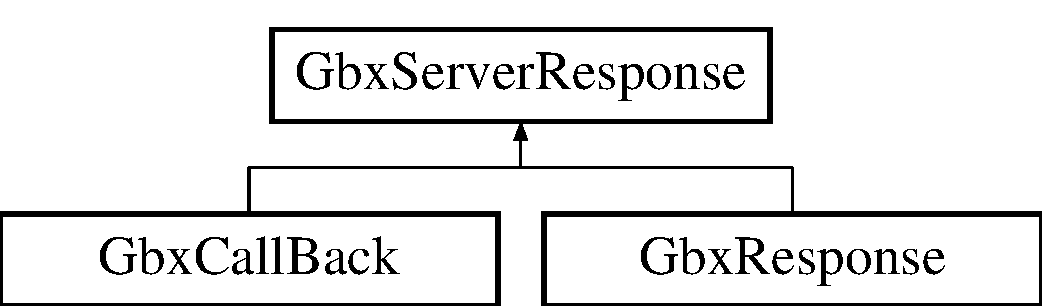
\includegraphics[height=2.000000cm]{classGbxServerResponse}
\end{center}
\end{figure}
\subsection*{Public Member Functions}
\begin{DoxyCompactItemize}
\item 
\hyperlink{classGbxServerResponse_a2198b6f6ca6b7da1ffd7bfa9a516d8b2}{Gbx\-Server\-Response} ()
\begin{DoxyCompactList}\small\item\em Empty constructor. \end{DoxyCompactList}\item 
\hyperlink{classGbxServerResponse_ad2a02192f5389a0fe10ea27cb24adedc}{$\sim$\-Gbx\-Server\-Response} ()
\item 
void \hyperlink{classGbxServerResponse_a1896da1a88aa07336829de953abe7364}{Set\-Raw} (char $\ast$response)
\begin{DoxyCompactList}\small\item\em Sets the raw message value. \end{DoxyCompactList}\item 
char $\ast$ \hyperlink{classGbxServerResponse_a3105f299a4f6a0d997f909415a467fd5}{Get\-Raw} ()
\begin{DoxyCompactList}\small\item\em Returns raw response (X\-M\-L). \end{DoxyCompactList}\item 
std\-::vector\\*
$<$ \hyperlink{classGbxResponseParameter}{Gbx\-Response\-Parameter} $>$ $\ast$ \hyperlink{classGbxServerResponse_ab791b8d9edb964b909d3c70753549668}{Get\-Parameters} ()
\begin{DoxyCompactList}\small\item\em Returns the extracted parameters. \end{DoxyCompactList}\end{DoxyCompactItemize}
\subsection*{Protected Member Functions}
\begin{DoxyCompactItemize}
\item 
\hyperlink{classGbxResponseParameter}{Gbx\-Response\-Parameter} \hyperlink{classGbxServerResponse_a22433a652ce9d4c7e9b834aa60c93c37}{extract\-Param} (pugi\-::xml\-\_\-node param)
\begin{DoxyCompactList}\small\item\em Extracts parameters from the raw data (X\-M\-L). \end{DoxyCompactList}\end{DoxyCompactItemize}
\subsection*{Protected Attributes}
\begin{DoxyCompactItemize}
\item 
char $\ast$ \hyperlink{classGbxServerResponse_aeee1fc539a5881334926e5c6789581bd}{data}
\begin{DoxyCompactList}\small\item\em Raw response data. \end{DoxyCompactList}\item 
std\-::vector\\*
$<$ \hyperlink{classGbxResponseParameter}{Gbx\-Response\-Parameter} $>$ $\ast$ \hyperlink{classGbxServerResponse_ad6fef5319c4da9461f4cd0d72d8b5ee8}{parameters} = new std\-::vector$<$\hyperlink{classGbxResponseParameter}{Gbx\-Response\-Parameter}$>$()
\begin{DoxyCompactList}\small\item\em List of parameters. \end{DoxyCompactList}\end{DoxyCompactItemize}


\subsection{Detailed Description}
Response from server, de-\/\-X\-M\-L-\/fies the response. 

\subsection{Constructor \& Destructor Documentation}
\hypertarget{classGbxServerResponse_a2198b6f6ca6b7da1ffd7bfa9a516d8b2}{\index{Gbx\-Server\-Response@{Gbx\-Server\-Response}!Gbx\-Server\-Response@{Gbx\-Server\-Response}}
\index{Gbx\-Server\-Response@{Gbx\-Server\-Response}!GbxServerResponse@{Gbx\-Server\-Response}}
\subsubsection[{Gbx\-Server\-Response}]{\setlength{\rightskip}{0pt plus 5cm}Gbx\-Server\-Response\-::\-Gbx\-Server\-Response (
\begin{DoxyParamCaption}
{}
\end{DoxyParamCaption}
)}}\label{classGbxServerResponse_a2198b6f6ca6b7da1ffd7bfa9a516d8b2}


Empty constructor. 

\hypertarget{classGbxServerResponse_ad2a02192f5389a0fe10ea27cb24adedc}{\index{Gbx\-Server\-Response@{Gbx\-Server\-Response}!$\sim$\-Gbx\-Server\-Response@{$\sim$\-Gbx\-Server\-Response}}
\index{$\sim$\-Gbx\-Server\-Response@{$\sim$\-Gbx\-Server\-Response}!GbxServerResponse@{Gbx\-Server\-Response}}
\subsubsection[{$\sim$\-Gbx\-Server\-Response}]{\setlength{\rightskip}{0pt plus 5cm}Gbx\-Server\-Response\-::$\sim$\-Gbx\-Server\-Response (
\begin{DoxyParamCaption}
{}
\end{DoxyParamCaption}
)}}\label{classGbxServerResponse_ad2a02192f5389a0fe10ea27cb24adedc}
Delets and nullifies the parameters. 

\subsection{Member Function Documentation}
\hypertarget{classGbxServerResponse_a22433a652ce9d4c7e9b834aa60c93c37}{\index{Gbx\-Server\-Response@{Gbx\-Server\-Response}!extract\-Param@{extract\-Param}}
\index{extract\-Param@{extract\-Param}!GbxServerResponse@{Gbx\-Server\-Response}}
\subsubsection[{extract\-Param}]{\setlength{\rightskip}{0pt plus 5cm}{\bf Gbx\-Response\-Parameter} Gbx\-Server\-Response\-::extract\-Param (
\begin{DoxyParamCaption}
\item[{pugi\-::xml\-\_\-node}]{param}
\end{DoxyParamCaption}
)\hspace{0.3cm}{\ttfamily [protected]}}}\label{classGbxServerResponse_a22433a652ce9d4c7e9b834aa60c93c37}


Extracts parameters from the raw data (X\-M\-L). 

\hypertarget{classGbxServerResponse_ab791b8d9edb964b909d3c70753549668}{\index{Gbx\-Server\-Response@{Gbx\-Server\-Response}!Get\-Parameters@{Get\-Parameters}}
\index{Get\-Parameters@{Get\-Parameters}!GbxServerResponse@{Gbx\-Server\-Response}}
\subsubsection[{Get\-Parameters}]{\setlength{\rightskip}{0pt plus 5cm}std\-::vector$<$ {\bf Gbx\-Response\-Parameter} $>$ $\ast$ Gbx\-Server\-Response\-::\-Get\-Parameters (
\begin{DoxyParamCaption}
{}
\end{DoxyParamCaption}
)}}\label{classGbxServerResponse_ab791b8d9edb964b909d3c70753549668}


Returns the extracted parameters. 

\hypertarget{classGbxServerResponse_a3105f299a4f6a0d997f909415a467fd5}{\index{Gbx\-Server\-Response@{Gbx\-Server\-Response}!Get\-Raw@{Get\-Raw}}
\index{Get\-Raw@{Get\-Raw}!GbxServerResponse@{Gbx\-Server\-Response}}
\subsubsection[{Get\-Raw}]{\setlength{\rightskip}{0pt plus 5cm}char $\ast$ Gbx\-Server\-Response\-::\-Get\-Raw (
\begin{DoxyParamCaption}
{}
\end{DoxyParamCaption}
)}}\label{classGbxServerResponse_a3105f299a4f6a0d997f909415a467fd5}


Returns raw response (X\-M\-L). 

\hypertarget{classGbxServerResponse_a1896da1a88aa07336829de953abe7364}{\index{Gbx\-Server\-Response@{Gbx\-Server\-Response}!Set\-Raw@{Set\-Raw}}
\index{Set\-Raw@{Set\-Raw}!GbxServerResponse@{Gbx\-Server\-Response}}
\subsubsection[{Set\-Raw}]{\setlength{\rightskip}{0pt plus 5cm}void Gbx\-Server\-Response\-::\-Set\-Raw (
\begin{DoxyParamCaption}
\item[{char $\ast$}]{response}
\end{DoxyParamCaption}
)}}\label{classGbxServerResponse_a1896da1a88aa07336829de953abe7364}


Sets the raw message value. 


\begin{DoxyParams}{Parameters}
{\em response} & Raw response from server (X\-M\-L). \\
\hline
\end{DoxyParams}


\subsection{Member Data Documentation}
\hypertarget{classGbxServerResponse_aeee1fc539a5881334926e5c6789581bd}{\index{Gbx\-Server\-Response@{Gbx\-Server\-Response}!data@{data}}
\index{data@{data}!GbxServerResponse@{Gbx\-Server\-Response}}
\subsubsection[{data}]{\setlength{\rightskip}{0pt plus 5cm}char$\ast$ Gbx\-Server\-Response\-::data\hspace{0.3cm}{\ttfamily [protected]}}}\label{classGbxServerResponse_aeee1fc539a5881334926e5c6789581bd}


Raw response data. 

\hypertarget{classGbxServerResponse_ad6fef5319c4da9461f4cd0d72d8b5ee8}{\index{Gbx\-Server\-Response@{Gbx\-Server\-Response}!parameters@{parameters}}
\index{parameters@{parameters}!GbxServerResponse@{Gbx\-Server\-Response}}
\subsubsection[{parameters}]{\setlength{\rightskip}{0pt plus 5cm}std\-::vector$<${\bf Gbx\-Response\-Parameter}$>$$\ast$ Gbx\-Server\-Response\-::parameters = new std\-::vector$<${\bf Gbx\-Response\-Parameter}$>$()\hspace{0.3cm}{\ttfamily [protected]}}}\label{classGbxServerResponse_ad6fef5319c4da9461f4cd0d72d8b5ee8}


List of parameters. 



The documentation for this class was generated from the following files\-:\begin{DoxyCompactItemize}
\item 
/home/travis/build/\-The\-Maximum/mania-\/pp/src/\-Gbx\-Remote/\-Server\-Response/\hyperlink{GbxServerResponse_8h}{Gbx\-Server\-Response.\-h}\item 
/home/travis/build/\-The\-Maximum/mania-\/pp/src/\-Gbx\-Remote/\-Server\-Response/\hyperlink{GbxServerResponse_8cpp}{Gbx\-Server\-Response.\-cpp}\end{DoxyCompactItemize}

\hypertarget{classHex}{\section{Hex Class Reference}
\label{classHex}\index{Hex@{Hex}}
}


Utility to print char arrays/pointers as hexadecimal values.  




{\ttfamily \#include $<$Hex.\-h$>$}

\subsection*{Static Public Member Functions}
\begin{DoxyCompactItemize}
\item 
static void \hyperlink{classHex_a875b48852fbd0032d85d01286d8653c1}{Print} (char message\mbox{[}$\,$\mbox{]}, int message\-Length)
\begin{DoxyCompactList}\small\item\em Prints char array as hexadecimal values. \end{DoxyCompactList}\item 
static void \hyperlink{classHex_a7a955b79027e7bb270b96d0f13e26043}{Print} (char $\ast$data)
\begin{DoxyCompactList}\small\item\em Prints char pointer as hexadecimal values. \end{DoxyCompactList}\end{DoxyCompactItemize}


\subsection{Detailed Description}
Utility to print char arrays/pointers as hexadecimal values. 

\subsection{Member Function Documentation}
\hypertarget{classHex_a875b48852fbd0032d85d01286d8653c1}{\index{Hex@{Hex}!Print@{Print}}
\index{Print@{Print}!Hex@{Hex}}
\subsubsection[{Print}]{\setlength{\rightskip}{0pt plus 5cm}static void Hex\-::\-Print (
\begin{DoxyParamCaption}
\item[{char}]{message\mbox{[}$\,$\mbox{]}, }
\item[{int}]{message\-Length}
\end{DoxyParamCaption}
)\hspace{0.3cm}{\ttfamily [inline]}, {\ttfamily [static]}}}\label{classHex_a875b48852fbd0032d85d01286d8653c1}


Prints char array as hexadecimal values. 

For printing the char array as hexadecimal, it uses the std\-::hex option. The char array is casted and printed char by char.


\begin{DoxyParams}{Parameters}
{\em message} & Char array with message to be displayed. \\
\hline
{\em message\-Length} & Length of the char array. \\
\hline
\end{DoxyParams}
\hypertarget{classHex_a7a955b79027e7bb270b96d0f13e26043}{\index{Hex@{Hex}!Print@{Print}}
\index{Print@{Print}!Hex@{Hex}}
\subsubsection[{Print}]{\setlength{\rightskip}{0pt plus 5cm}static void Hex\-::\-Print (
\begin{DoxyParamCaption}
\item[{char $\ast$}]{data}
\end{DoxyParamCaption}
)\hspace{0.3cm}{\ttfamily [inline]}, {\ttfamily [static]}}}\label{classHex_a7a955b79027e7bb270b96d0f13e26043}


Prints char pointer as hexadecimal values. 

Casts the pointer to a char array and uses the char array version of the function.


\begin{DoxyParams}{Parameters}
{\em data} & Char pointer with message to be displayed. \\
\hline
\end{DoxyParams}


The documentation for this class was generated from the following file\-:\begin{DoxyCompactItemize}
\item 
/home/travis/build/\-The\-Maximum/mania-\/pp/src/\-Utils/\hyperlink{Hex_8h}{Hex.\-h}\end{DoxyCompactItemize}

\hypertarget{classLogging}{\section{Logging Class Reference}
\label{classLogging}\index{Logging@{Logging}}
}


Utility to print information to the console.  




{\ttfamily \#include $<$Logging.\-h$>$}

\subsection*{Static Public Member Functions}
\begin{DoxyCompactItemize}
\item 
static void \hyperlink{classLogging_a171703bedcbf215f0e6334f29c8281b5}{Print\-Error} (\hyperlink{structGbxError}{Gbx\-Error} $\ast$error)
\begin{DoxyCompactList}\small\item\em Prints error to console. \end{DoxyCompactList}\item 
static void \hyperlink{classLogging_ac1397db1b8ea6625f7dd2616f530cd7d}{Print\-Error} (int number, std\-::string message)
\begin{DoxyCompactList}\small\item\em Prints error to console. \end{DoxyCompactList}\item 
\hypertarget{classLogging_a889f2ad8f991afdf0959cb1cad736fa7}{static void \hyperlink{classLogging_a889f2ad8f991afdf0959cb1cad736fa7}{Print\-O\-K\-Flush} ()}\label{classLogging_a889f2ad8f991afdf0959cb1cad736fa7}

\begin{DoxyCompactList}\small\item\em Prints O\-K. in \mbox{[} \mbox{]}-\/spaces in console. \end{DoxyCompactList}\item 
\hypertarget{classLogging_add0483bd14aef74ec988606cd7dbfc4b}{static void \hyperlink{classLogging_add0483bd14aef74ec988606cd7dbfc4b}{Print\-Failed\-Flush} ()}\label{classLogging_add0483bd14aef74ec988606cd7dbfc4b}

\begin{DoxyCompactList}\small\item\em Prints Failed! in \mbox{[} \mbox{]}-\/spaces in console. \end{DoxyCompactList}\item 
static void \hyperlink{classLogging_a1f8609052e40055fb9ef3ddd40d0620e}{Print\-Parameter} (\hyperlink{classGbxResponseParameter}{Gbx\-Response\-Parameter} parameter, int param\-Id, std\-::string spaces=\char`\"{}    \char`\"{}, std\-::string parameter\-Name=\char`\"{}\char`\"{})
\begin{DoxyCompactList}\small\item\em Prints a \hyperlink{classGbxResponseParameter}{Gbx\-Response\-Parameter} (for D\-E\-B\-U\-G purposes). \end{DoxyCompactList}\end{DoxyCompactItemize}


\subsection{Detailed Description}
Utility to print information to the console. 

\subsection{Member Function Documentation}
\hypertarget{classLogging_a171703bedcbf215f0e6334f29c8281b5}{\index{Logging@{Logging}!Print\-Error@{Print\-Error}}
\index{Print\-Error@{Print\-Error}!Logging@{Logging}}
\subsubsection[{Print\-Error}]{\setlength{\rightskip}{0pt plus 5cm}static void Logging\-::\-Print\-Error (
\begin{DoxyParamCaption}
\item[{{\bf Gbx\-Error} $\ast$}]{error}
\end{DoxyParamCaption}
)\hspace{0.3cm}{\ttfamily [inline]}, {\ttfamily [static]}}}\label{classLogging_a171703bedcbf215f0e6334f29c8281b5}


Prints error to console. 


\begin{DoxyParams}{Parameters}
{\em error} & Error structure. \\
\hline
\end{DoxyParams}
\hypertarget{classLogging_ac1397db1b8ea6625f7dd2616f530cd7d}{\index{Logging@{Logging}!Print\-Error@{Print\-Error}}
\index{Print\-Error@{Print\-Error}!Logging@{Logging}}
\subsubsection[{Print\-Error}]{\setlength{\rightskip}{0pt plus 5cm}static void Logging\-::\-Print\-Error (
\begin{DoxyParamCaption}
\item[{int}]{number, }
\item[{std\-::string}]{message}
\end{DoxyParamCaption}
)\hspace{0.3cm}{\ttfamily [inline]}, {\ttfamily [static]}}}\label{classLogging_ac1397db1b8ea6625f7dd2616f530cd7d}


Prints error to console. 


\begin{DoxyParams}{Parameters}
{\em number} & Error number. \\
\hline
{\em message} & Error message. \\
\hline
\end{DoxyParams}
\hypertarget{classLogging_a1f8609052e40055fb9ef3ddd40d0620e}{\index{Logging@{Logging}!Print\-Parameter@{Print\-Parameter}}
\index{Print\-Parameter@{Print\-Parameter}!Logging@{Logging}}
\subsubsection[{Print\-Parameter}]{\setlength{\rightskip}{0pt plus 5cm}static void Logging\-::\-Print\-Parameter (
\begin{DoxyParamCaption}
\item[{{\bf Gbx\-Response\-Parameter}}]{parameter, }
\item[{int}]{param\-Id, }
\item[{std\-::string}]{spaces = {\ttfamily \char`\"{}~~~~\char`\"{}}, }
\item[{std\-::string}]{parameter\-Name = {\ttfamily \char`\"{}\char`\"{}}}
\end{DoxyParamCaption}
)\hspace{0.3cm}{\ttfamily [inline]}, {\ttfamily [static]}}}\label{classLogging_a1f8609052e40055fb9ef3ddd40d0620e}


Prints a \hyperlink{classGbxResponseParameter}{Gbx\-Response\-Parameter} (for D\-E\-B\-U\-G purposes). 


\begin{DoxyParams}{Parameters}
{\em parameter} & Parameter to be printed. \\
\hline
{\em param\-Id} & Number of the parameter. \\
\hline
{\em spaces} & Spaces to be put before the parameter information. \\
\hline
{\em parameter\-Name} & Name of the parameter (struct value only). \\
\hline
\end{DoxyParams}


The documentation for this class was generated from the following file\-:\begin{DoxyCompactItemize}
\item 
/home/travis/build/\-The\-Maximum/mania-\/pp/src/\-Utils/Logging.\-h\end{DoxyCompactItemize}

\hypertarget{classManiaPP}{\section{Mania\-P\-P Class Reference}
\label{classManiaPP}\index{Mania\-P\-P@{Mania\-P\-P}}
}


Main class.  




{\ttfamily \#include $<$Mania\-P\-P.\-h$>$}

\subsection*{Public Member Functions}
\begin{DoxyCompactItemize}
\item 
\hyperlink{classManiaPP_ae56f6623dc89f2c0b75bec631cfc2d19}{Mania\-P\-P} ()
\begin{DoxyCompactList}\small\item\em Sets up the several variables needed to run the software. \end{DoxyCompactList}\item 
\hyperlink{classManiaPP_a1c78c3b51db550609011fb6fdcb26ec8}{$\sim$\-Mania\-P\-P} ()
\begin{DoxyCompactList}\small\item\em Destructs the pointers in the main class. \end{DoxyCompactList}\item 
bool \hyperlink{classManiaPP_a22561171876e54dbf633c70d9924c06a}{Connect\-To\-Server} ()
\begin{DoxyCompactList}\small\item\em Connects and authenticates with the server. \end{DoxyCompactList}\item 
void \hyperlink{classManiaPP_a56d2774a29f21b3a164ae1f7ea6bd88b}{Print\-Server\-Info} ()
\begin{DoxyCompactList}\small\item\em Prints information about the server. \end{DoxyCompactList}\item 
void \hyperlink{classManiaPP_a8dff9e8e3835c3cac0df105a7bcce43c}{Main\-Loop} ()
\begin{DoxyCompactList}\small\item\em Performing our tasks ... \end{DoxyCompactList}\item 
void \hyperlink{classManiaPP_a87fd53fffe4a1840834a90ab575f5ce6}{Terminate} ()
\begin{DoxyCompactList}\small\item\em Disconnects the software from the server. \end{DoxyCompactList}\item 
void \hyperlink{classManiaPP_a3548cbafbf949dbb9d210c08adb5f7de}{Print\-Parameter} (\hyperlink{classGbxResponseParameter}{Gbx\-Response\-Parameter} parameter, int param\-Id, std\-::string spaces=\char`\"{}    \char`\"{})
\end{DoxyCompactItemize}
\subsection*{Private Member Functions}
\begin{DoxyCompactItemize}
\item 
void \hyperlink{classManiaPP_aede94c0b982250de19186d447542e479}{retrieve\-Player\-List} ()
\begin{DoxyCompactList}\small\item\em Gets a list of current players from the server. \end{DoxyCompactList}\item 
void \hyperlink{classManiaPP_a18582fa28b259c22a8a8d526af62123a}{retrieve\-Map\-List} ()
\begin{DoxyCompactList}\small\item\em Gets a list of current maps from the server. \end{DoxyCompactList}\end{DoxyCompactItemize}
\subsection*{Private Attributes}
\begin{DoxyCompactItemize}
\item 
\hyperlink{classConfig}{Config} $\ast$ \hyperlink{classManiaPP_a9a91437fa70afd52c2dce19298888e36}{config}
\begin{DoxyCompactList}\small\item\em Contains the configuration for the software. \end{DoxyCompactList}\item 
\hyperlink{classLogging}{Logging} $\ast$ \hyperlink{classManiaPP_aa4cea090301bdf0bf652ad377e7b01c0}{logging}
\begin{DoxyCompactList}\small\item\em Contains functions to log information. \end{DoxyCompactList}\item 
\hyperlink{classGbxRemote}{Gbx\-Remote} $\ast$ \hyperlink{classManiaPP_ab81311d6901990cb99a7a30e0cbaab11}{server}
\begin{DoxyCompactList}\small\item\em Contains the connection with the server and its methods. \end{DoxyCompactList}\item 
std\-::map$<$ std\-::string, \hyperlink{structPlayer}{Player} $>$ $\ast$ \hyperlink{classManiaPP_a45712ccfa91b20242b39cb1164d305d8}{players}
\begin{DoxyCompactList}\small\item\em Contains the list of players currently on the server. \end{DoxyCompactList}\item 
std\-::map$<$ std\-::string, \hyperlink{structMap}{Map} $>$ $\ast$ \hyperlink{classManiaPP_a903ccf13c65b15c99595cb571214799d}{maps}
\begin{DoxyCompactList}\small\item\em Contains the list of players currently on the server. \end{DoxyCompactList}\end{DoxyCompactItemize}


\subsection{Detailed Description}
Main class. 

\subsection{Constructor \& Destructor Documentation}
\hypertarget{classManiaPP_ae56f6623dc89f2c0b75bec631cfc2d19}{\index{Mania\-P\-P@{Mania\-P\-P}!Mania\-P\-P@{Mania\-P\-P}}
\index{Mania\-P\-P@{Mania\-P\-P}!ManiaPP@{Mania\-P\-P}}
\subsubsection[{Mania\-P\-P}]{\setlength{\rightskip}{0pt plus 5cm}Mania\-P\-P\-::\-Mania\-P\-P (
\begin{DoxyParamCaption}
{}
\end{DoxyParamCaption}
)}}\label{classManiaPP_ae56f6623dc89f2c0b75bec631cfc2d19}


Sets up the several variables needed to run the software. 

\hypertarget{classManiaPP_a1c78c3b51db550609011fb6fdcb26ec8}{\index{Mania\-P\-P@{Mania\-P\-P}!$\sim$\-Mania\-P\-P@{$\sim$\-Mania\-P\-P}}
\index{$\sim$\-Mania\-P\-P@{$\sim$\-Mania\-P\-P}!ManiaPP@{Mania\-P\-P}}
\subsubsection[{$\sim$\-Mania\-P\-P}]{\setlength{\rightskip}{0pt plus 5cm}Mania\-P\-P\-::$\sim$\-Mania\-P\-P (
\begin{DoxyParamCaption}
{}
\end{DoxyParamCaption}
)}}\label{classManiaPP_a1c78c3b51db550609011fb6fdcb26ec8}


Destructs the pointers in the main class. 



\subsection{Member Function Documentation}
\hypertarget{classManiaPP_a22561171876e54dbf633c70d9924c06a}{\index{Mania\-P\-P@{Mania\-P\-P}!Connect\-To\-Server@{Connect\-To\-Server}}
\index{Connect\-To\-Server@{Connect\-To\-Server}!ManiaPP@{Mania\-P\-P}}
\subsubsection[{Connect\-To\-Server}]{\setlength{\rightskip}{0pt plus 5cm}bool Mania\-P\-P\-::\-Connect\-To\-Server (
\begin{DoxyParamCaption}
{}
\end{DoxyParamCaption}
)}}\label{classManiaPP_a22561171876e54dbf633c70d9924c06a}


Connects and authenticates with the server. 

\hypertarget{classManiaPP_a8dff9e8e3835c3cac0df105a7bcce43c}{\index{Mania\-P\-P@{Mania\-P\-P}!Main\-Loop@{Main\-Loop}}
\index{Main\-Loop@{Main\-Loop}!ManiaPP@{Mania\-P\-P}}
\subsubsection[{Main\-Loop}]{\setlength{\rightskip}{0pt plus 5cm}void Mania\-P\-P\-::\-Main\-Loop (
\begin{DoxyParamCaption}
{}
\end{DoxyParamCaption}
)}}\label{classManiaPP_a8dff9e8e3835c3cac0df105a7bcce43c}


Performing our tasks ... 

\hypertarget{classManiaPP_a3548cbafbf949dbb9d210c08adb5f7de}{\index{Mania\-P\-P@{Mania\-P\-P}!Print\-Parameter@{Print\-Parameter}}
\index{Print\-Parameter@{Print\-Parameter}!ManiaPP@{Mania\-P\-P}}
\subsubsection[{Print\-Parameter}]{\setlength{\rightskip}{0pt plus 5cm}void Mania\-P\-P\-::\-Print\-Parameter (
\begin{DoxyParamCaption}
\item[{{\bf Gbx\-Response\-Parameter}}]{parameter, }
\item[{int}]{param\-Id, }
\item[{std\-::string}]{spaces = {\ttfamily \char`\"{}~~~~\char`\"{}}}
\end{DoxyParamCaption}
)}}\label{classManiaPP_a3548cbafbf949dbb9d210c08adb5f7de}
\hypertarget{classManiaPP_a56d2774a29f21b3a164ae1f7ea6bd88b}{\index{Mania\-P\-P@{Mania\-P\-P}!Print\-Server\-Info@{Print\-Server\-Info}}
\index{Print\-Server\-Info@{Print\-Server\-Info}!ManiaPP@{Mania\-P\-P}}
\subsubsection[{Print\-Server\-Info}]{\setlength{\rightskip}{0pt plus 5cm}void Mania\-P\-P\-::\-Print\-Server\-Info (
\begin{DoxyParamCaption}
{}
\end{DoxyParamCaption}
)}}\label{classManiaPP_a56d2774a29f21b3a164ae1f7ea6bd88b}


Prints information about the server. 

\hypertarget{classManiaPP_a18582fa28b259c22a8a8d526af62123a}{\index{Mania\-P\-P@{Mania\-P\-P}!retrieve\-Map\-List@{retrieve\-Map\-List}}
\index{retrieve\-Map\-List@{retrieve\-Map\-List}!ManiaPP@{Mania\-P\-P}}
\subsubsection[{retrieve\-Map\-List}]{\setlength{\rightskip}{0pt plus 5cm}void Mania\-P\-P\-::retrieve\-Map\-List (
\begin{DoxyParamCaption}
{}
\end{DoxyParamCaption}
)\hspace{0.3cm}{\ttfamily [private]}}}\label{classManiaPP_a18582fa28b259c22a8a8d526af62123a}


Gets a list of current maps from the server. 

\hypertarget{classManiaPP_aede94c0b982250de19186d447542e479}{\index{Mania\-P\-P@{Mania\-P\-P}!retrieve\-Player\-List@{retrieve\-Player\-List}}
\index{retrieve\-Player\-List@{retrieve\-Player\-List}!ManiaPP@{Mania\-P\-P}}
\subsubsection[{retrieve\-Player\-List}]{\setlength{\rightskip}{0pt plus 5cm}void Mania\-P\-P\-::retrieve\-Player\-List (
\begin{DoxyParamCaption}
{}
\end{DoxyParamCaption}
)\hspace{0.3cm}{\ttfamily [private]}}}\label{classManiaPP_aede94c0b982250de19186d447542e479}


Gets a list of current players from the server. 

\hypertarget{classManiaPP_a87fd53fffe4a1840834a90ab575f5ce6}{\index{Mania\-P\-P@{Mania\-P\-P}!Terminate@{Terminate}}
\index{Terminate@{Terminate}!ManiaPP@{Mania\-P\-P}}
\subsubsection[{Terminate}]{\setlength{\rightskip}{0pt plus 5cm}void Mania\-P\-P\-::\-Terminate (
\begin{DoxyParamCaption}
{}
\end{DoxyParamCaption}
)}}\label{classManiaPP_a87fd53fffe4a1840834a90ab575f5ce6}


Disconnects the software from the server. 



\subsection{Member Data Documentation}
\hypertarget{classManiaPP_a9a91437fa70afd52c2dce19298888e36}{\index{Mania\-P\-P@{Mania\-P\-P}!config@{config}}
\index{config@{config}!ManiaPP@{Mania\-P\-P}}
\subsubsection[{config}]{\setlength{\rightskip}{0pt plus 5cm}{\bf Config}$\ast$ Mania\-P\-P\-::config\hspace{0.3cm}{\ttfamily [private]}}}\label{classManiaPP_a9a91437fa70afd52c2dce19298888e36}


Contains the configuration for the software. 

\hypertarget{classManiaPP_aa4cea090301bdf0bf652ad377e7b01c0}{\index{Mania\-P\-P@{Mania\-P\-P}!logging@{logging}}
\index{logging@{logging}!ManiaPP@{Mania\-P\-P}}
\subsubsection[{logging}]{\setlength{\rightskip}{0pt plus 5cm}{\bf Logging}$\ast$ Mania\-P\-P\-::logging\hspace{0.3cm}{\ttfamily [private]}}}\label{classManiaPP_aa4cea090301bdf0bf652ad377e7b01c0}


Contains functions to log information. 

\hypertarget{classManiaPP_a903ccf13c65b15c99595cb571214799d}{\index{Mania\-P\-P@{Mania\-P\-P}!maps@{maps}}
\index{maps@{maps}!ManiaPP@{Mania\-P\-P}}
\subsubsection[{maps}]{\setlength{\rightskip}{0pt plus 5cm}std\-::map$<$std\-::string, {\bf Map}$>$$\ast$ Mania\-P\-P\-::maps\hspace{0.3cm}{\ttfamily [private]}}}\label{classManiaPP_a903ccf13c65b15c99595cb571214799d}


Contains the list of players currently on the server. 

\hypertarget{classManiaPP_a45712ccfa91b20242b39cb1164d305d8}{\index{Mania\-P\-P@{Mania\-P\-P}!players@{players}}
\index{players@{players}!ManiaPP@{Mania\-P\-P}}
\subsubsection[{players}]{\setlength{\rightskip}{0pt plus 5cm}std\-::map$<$std\-::string, {\bf Player}$>$$\ast$ Mania\-P\-P\-::players\hspace{0.3cm}{\ttfamily [private]}}}\label{classManiaPP_a45712ccfa91b20242b39cb1164d305d8}


Contains the list of players currently on the server. 

\hypertarget{classManiaPP_ab81311d6901990cb99a7a30e0cbaab11}{\index{Mania\-P\-P@{Mania\-P\-P}!server@{server}}
\index{server@{server}!ManiaPP@{Mania\-P\-P}}
\subsubsection[{server}]{\setlength{\rightskip}{0pt plus 5cm}{\bf Gbx\-Remote}$\ast$ Mania\-P\-P\-::server\hspace{0.3cm}{\ttfamily [private]}}}\label{classManiaPP_ab81311d6901990cb99a7a30e0cbaab11}


Contains the connection with the server and its methods. 



The documentation for this class was generated from the following files\-:\begin{DoxyCompactItemize}
\item 
/home/travis/build/\-The\-Maximum/mania-\/pp/src/\hyperlink{ManiaPP_8h}{Mania\-P\-P.\-h}\item 
/home/travis/build/\-The\-Maximum/mania-\/pp/src/\hyperlink{ManiaPP_8cpp}{Mania\-P\-P.\-cpp}\end{DoxyCompactItemize}

\hypertarget{structPlayer}{\section{Player Struct Reference}
\label{structPlayer}\index{Player@{Player}}
}


Contains all information about a player in easy-\/to-\/use format.  




{\ttfamily \#include $<$Player.\-h$>$}

\subsection*{Public Member Functions}
\begin{DoxyCompactItemize}
\item 
\hypertarget{structPlayer_affe0cc3cb714f6deb4e62f0c0d3f1fd8}{\hyperlink{structPlayer_affe0cc3cb714f6deb4e62f0c0d3f1fd8}{Player} ()}\label{structPlayer_affe0cc3cb714f6deb4e62f0c0d3f1fd8}

\begin{DoxyCompactList}\small\item\em Constructs a \hyperlink{structPlayer}{Player} object without input. \end{DoxyCompactList}\item 
\hyperlink{structPlayer_adf15eb006b535a4e1b72b419021f1f11}{Player} (std\-::map$<$ std\-::string, \hyperlink{classGbxResponseParameter}{Gbx\-Response\-Parameter} $>$ server\-Struct)
\begin{DoxyCompactList}\small\item\em Formats a server response into a usable form. \end{DoxyCompactList}\item 
void \hyperlink{structPlayer_afa8ea116543628f0129b5fb1cb17f2ef}{Set\-Basic} (std\-::map$<$ std\-::string, \hyperlink{classGbxResponseParameter}{Gbx\-Response\-Parameter} $>$ server\-Struct)
\begin{DoxyCompactList}\small\item\em Formats a server response into a usable form. \end{DoxyCompactList}\item 
void \hyperlink{structPlayer_a4e7c4a5bfc6fe42e23069a79f495b461}{Player\-Detailed} (std\-::map$<$ std\-::string, \hyperlink{classGbxResponseParameter}{Gbx\-Response\-Parameter} $>$ server\-Struct)
\begin{DoxyCompactList}\small\item\em Formats a server response into a usable form. \end{DoxyCompactList}\item 
void \hyperlink{structPlayer_a8541713f4fceaf4d03745e9407c3c303}{Set\-Id} (int id)
\begin{DoxyCompactList}\small\item\em Set database identifier value. \end{DoxyCompactList}\end{DoxyCompactItemize}
\subsection*{Public Attributes}
\begin{DoxyCompactItemize}
\item 
\hypertarget{structPlayer_a27cd3355e96dc3842d4f91b859673e0c}{int \hyperlink{structPlayer_a27cd3355e96dc3842d4f91b859673e0c}{Id} = 0}\label{structPlayer_a27cd3355e96dc3842d4f91b859673e0c}

\begin{DoxyCompactList}\small\item\em \hyperlink{structPlayer}{Player} identifier (on database). \end{DoxyCompactList}\item 
\hypertarget{structPlayer_aa6efdb36b3a3618f26bf85c3a9b216d8}{std\-::vector$<$ int $>$ \hyperlink{structPlayer_aa6efdb36b3a3618f26bf85c3a9b216d8}{Current\-Checkpoints}}\label{structPlayer_aa6efdb36b3a3618f26bf85c3a9b216d8}

\begin{DoxyCompactList}\small\item\em Checkpoint passes on current try. \end{DoxyCompactList}\item 
\hypertarget{structPlayer_a8c221131108dd948b17c6eb68cd1b4db}{time\-\_\-t \hyperlink{structPlayer_a8c221131108dd948b17c6eb68cd1b4db}{Joined\-At}}\label{structPlayer_a8c221131108dd948b17c6eb68cd1b4db}

\begin{DoxyCompactList}\small\item\em The timestamp on join. \end{DoxyCompactList}\item 
\hypertarget{structPlayer_aa83b14faf5c02be9dd38c6963b245916}{Permission \hyperlink{structPlayer_aa83b14faf5c02be9dd38c6963b245916}{Access\-Level} = User}\label{structPlayer_aa83b14faf5c02be9dd38c6963b245916}

\begin{DoxyCompactList}\small\item\em Permission level. \end{DoxyCompactList}\item 
\hypertarget{structPlayer_a6a71d7d9837a0a12e52ca47930965e0f}{int \hyperlink{structPlayer_a6a71d7d9837a0a12e52ca47930965e0f}{Player\-Id}}\label{structPlayer_a6a71d7d9837a0a12e52ca47930965e0f}

\begin{DoxyCompactList}\small\item\em \hyperlink{structPlayer}{Player} identifier (on server). \end{DoxyCompactList}\item 
\hypertarget{structPlayer_a350919664ba73d6d6cd6d03bd2a5cacd}{int \hyperlink{structPlayer_a350919664ba73d6d6cd6d03bd2a5cacd}{Team\-Id}}\label{structPlayer_a350919664ba73d6d6cd6d03bd2a5cacd}

\begin{DoxyCompactList}\small\item\em Team identifier (on server). \end{DoxyCompactList}\item 
\hypertarget{structPlayer_a38398818d43e186aa982a788744792d7}{std\-::string \hyperlink{structPlayer_a38398818d43e186aa982a788744792d7}{Login}}\label{structPlayer_a38398818d43e186aa982a788744792d7}

\begin{DoxyCompactList}\small\item\em \hyperlink{structPlayer}{Player} login. \end{DoxyCompactList}\item 
\hypertarget{structPlayer_a553cc1b0aa79108b511ba408210582cf}{std\-::string \hyperlink{structPlayer_a553cc1b0aa79108b511ba408210582cf}{Nick\-Name}}\label{structPlayer_a553cc1b0aa79108b511ba408210582cf}

\begin{DoxyCompactList}\small\item\em \hyperlink{structPlayer}{Player} nickname. \end{DoxyCompactList}\item 
\hypertarget{structPlayer_a2037601661fb699454a88b5649485b30}{int \hyperlink{structPlayer_a2037601661fb699454a88b5649485b30}{Spectator\-Status}}\label{structPlayer_a2037601661fb699454a88b5649485b30}

\begin{DoxyCompactList}\small\item\em Spectator status of player. \end{DoxyCompactList}\item 
\hypertarget{structPlayer_aa151b994eedc8ba67b3fd48905db5ac0}{int \hyperlink{structPlayer_aa151b994eedc8ba67b3fd48905db5ac0}{Flags}}\label{structPlayer_aa151b994eedc8ba67b3fd48905db5ac0}

\begin{DoxyCompactList}\small\item\em \hyperlink{structPlayer}{Player} flags. \end{DoxyCompactList}\item 
\hypertarget{structPlayer_a25fe69852f0e38f541ad615cd59877ef}{int \hyperlink{structPlayer_a25fe69852f0e38f541ad615cd59877ef}{Ladder\-Ranking}}\label{structPlayer_a25fe69852f0e38f541ad615cd59877ef}

\begin{DoxyCompactList}\small\item\em Current ladder ranking of the player. \end{DoxyCompactList}\item 
\hypertarget{structPlayer_a388787a2218deeaf7318f0fbbd3f5d0f}{std\-::string \hyperlink{structPlayer_a388787a2218deeaf7318f0fbbd3f5d0f}{I\-P\-Address}}\label{structPlayer_a388787a2218deeaf7318f0fbbd3f5d0f}

\begin{DoxyCompactList}\small\item\em I\-P Address of the player. \end{DoxyCompactList}\item 
\hypertarget{structPlayer_a7fcee993ceed3c2b737782bc549e11bf}{int \hyperlink{structPlayer_a7fcee993ceed3c2b737782bc549e11bf}{Download\-Rate}}\label{structPlayer_a7fcee993ceed3c2b737782bc549e11bf}

\begin{DoxyCompactList}\small\item\em Download rate in Kbps. \end{DoxyCompactList}\item 
\hypertarget{structPlayer_a28f9a31a54ac8ea0658a6b234523b29d}{int \hyperlink{structPlayer_a28f9a31a54ac8ea0658a6b234523b29d}{Upload\-Rate}}\label{structPlayer_a28f9a31a54ac8ea0658a6b234523b29d}

\begin{DoxyCompactList}\small\item\em Upload rate in Kbps. \end{DoxyCompactList}\item 
\hypertarget{structPlayer_a583abe4cc5985fc83bfed62362efa358}{std\-::string \hyperlink{structPlayer_a583abe4cc5985fc83bfed62362efa358}{Language}}\label{structPlayer_a583abe4cc5985fc83bfed62362efa358}

\begin{DoxyCompactList}\small\item\em Application language. \end{DoxyCompactList}\item 
\hypertarget{structPlayer_a61ba0e32d336f5cd1eb152addf6848d2}{bool \hyperlink{structPlayer_a61ba0e32d336f5cd1eb152addf6848d2}{Is\-Spectator}}\label{structPlayer_a61ba0e32d336f5cd1eb152addf6848d2}

\begin{DoxyCompactList}\small\item\em Is in spectatormode? \end{DoxyCompactList}\item 
\hypertarget{structPlayer_a76e8b5298bcbe9ff694b6ed490ef7ca5}{bool \hyperlink{structPlayer_a76e8b5298bcbe9ff694b6ed490ef7ca5}{Is\-In\-Official\-Mode}}\label{structPlayer_a76e8b5298bcbe9ff694b6ed490ef7ca5}

\begin{DoxyCompactList}\small\item\em Is in official mode? \end{DoxyCompactList}\item 
\hypertarget{structPlayer_ae275137c2fe689552ebde4d3b1e5f4ff}{std\-::string \hyperlink{structPlayer_ae275137c2fe689552ebde4d3b1e5f4ff}{Client\-Version}}\label{structPlayer_ae275137c2fe689552ebde4d3b1e5f4ff}

\begin{DoxyCompactList}\small\item\em Client version (f.\-e. 'v2015-\/06-\/18\-\_\-15\-\_\-10 (3.\-3.\-0)'). \end{DoxyCompactList}\item 
\hypertarget{structPlayer_af6acb51bf731275d73aa6cc55a8255a8}{std\-::string \hyperlink{structPlayer_af6acb51bf731275d73aa6cc55a8255a8}{Club\-Link}}\label{structPlayer_af6acb51bf731275d73aa6cc55a8255a8}

\begin{DoxyCompactList}\small\item\em Club U\-R\-L (website, entered by player). \end{DoxyCompactList}\item 
\hypertarget{structPlayer_a3da038886ddd825ebc9612b460ecd008}{std\-::string \hyperlink{structPlayer_a3da038886ddd825ebc9612b460ecd008}{Path}}\label{structPlayer_a3da038886ddd825ebc9612b460ecd008}

\begin{DoxyCompactList}\small\item\em \hyperlink{structPlayer}{Player} location without \char`\"{}world\char`\"{}. \end{DoxyCompactList}\item 
\hypertarget{structPlayer_aa04503994922157165081fa29bf4729d}{std\-::string \hyperlink{structPlayer_aa04503994922157165081fa29bf4729d}{Country}}\label{structPlayer_aa04503994922157165081fa29bf4729d}

\begin{DoxyCompactList}\small\item\em Path without continent. \end{DoxyCompactList}\end{DoxyCompactItemize}
\subsection*{Private Member Functions}
\begin{DoxyCompactItemize}
\item 
void \hyperlink{structPlayer_ac4666bfba77342a37f3ab3628b26acd0}{set\-Basic\-Info} (std\-::map$<$ std\-::string, \hyperlink{classGbxResponseParameter}{Gbx\-Response\-Parameter} $>$ server\-Struct)
\begin{DoxyCompactList}\small\item\em Sets the basic player information from the struct. \end{DoxyCompactList}\item 
void \hyperlink{structPlayer_a179183e86a0b9a4b808593be96d65391}{set\-Detailed\-Info} (std\-::map$<$ std\-::string, \hyperlink{classGbxResponseParameter}{Gbx\-Response\-Parameter} $>$ server\-Struct)
\begin{DoxyCompactList}\small\item\em Sets the detailed player information from the struct. \end{DoxyCompactList}\end{DoxyCompactItemize}


\subsection{Detailed Description}
Contains all information about a player in easy-\/to-\/use format. 

\subsection{Constructor \& Destructor Documentation}
\hypertarget{structPlayer_adf15eb006b535a4e1b72b419021f1f11}{\index{Player@{Player}!Player@{Player}}
\index{Player@{Player}!Player@{Player}}
\subsubsection[{Player}]{\setlength{\rightskip}{0pt plus 5cm}Player\-::\-Player (
\begin{DoxyParamCaption}
\item[{std\-::map$<$ std\-::string, {\bf Gbx\-Response\-Parameter} $>$}]{server\-Struct}
\end{DoxyParamCaption}
)\hspace{0.3cm}{\ttfamily [inline]}}}\label{structPlayer_adf15eb006b535a4e1b72b419021f1f11}


Formats a server response into a usable form. 


\begin{DoxyParams}{Parameters}
{\em server\-Struct} & The struct with player information received from the server. \\
\hline
\end{DoxyParams}


\subsection{Member Function Documentation}
\hypertarget{structPlayer_a4e7c4a5bfc6fe42e23069a79f495b461}{\index{Player@{Player}!Player\-Detailed@{Player\-Detailed}}
\index{Player\-Detailed@{Player\-Detailed}!Player@{Player}}
\subsubsection[{Player\-Detailed}]{\setlength{\rightskip}{0pt plus 5cm}void Player\-::\-Player\-Detailed (
\begin{DoxyParamCaption}
\item[{std\-::map$<$ std\-::string, {\bf Gbx\-Response\-Parameter} $>$}]{server\-Struct}
\end{DoxyParamCaption}
)\hspace{0.3cm}{\ttfamily [inline]}}}\label{structPlayer_a4e7c4a5bfc6fe42e23069a79f495b461}


Formats a server response into a usable form. 


\begin{DoxyParams}{Parameters}
{\em server\-Struct} & The struct with detailed player information received from the server. \\
\hline
\end{DoxyParams}
\hypertarget{structPlayer_afa8ea116543628f0129b5fb1cb17f2ef}{\index{Player@{Player}!Set\-Basic@{Set\-Basic}}
\index{Set\-Basic@{Set\-Basic}!Player@{Player}}
\subsubsection[{Set\-Basic}]{\setlength{\rightskip}{0pt plus 5cm}void Player\-::\-Set\-Basic (
\begin{DoxyParamCaption}
\item[{std\-::map$<$ std\-::string, {\bf Gbx\-Response\-Parameter} $>$}]{server\-Struct}
\end{DoxyParamCaption}
)\hspace{0.3cm}{\ttfamily [inline]}}}\label{structPlayer_afa8ea116543628f0129b5fb1cb17f2ef}


Formats a server response into a usable form. 


\begin{DoxyParams}{Parameters}
{\em server\-Struct} & The struct with player information received from the server. \\
\hline
\end{DoxyParams}
\hypertarget{structPlayer_ac4666bfba77342a37f3ab3628b26acd0}{\index{Player@{Player}!set\-Basic\-Info@{set\-Basic\-Info}}
\index{set\-Basic\-Info@{set\-Basic\-Info}!Player@{Player}}
\subsubsection[{set\-Basic\-Info}]{\setlength{\rightskip}{0pt plus 5cm}void Player\-::set\-Basic\-Info (
\begin{DoxyParamCaption}
\item[{std\-::map$<$ std\-::string, {\bf Gbx\-Response\-Parameter} $>$}]{server\-Struct}
\end{DoxyParamCaption}
)\hspace{0.3cm}{\ttfamily [inline]}, {\ttfamily [private]}}}\label{structPlayer_ac4666bfba77342a37f3ab3628b26acd0}


Sets the basic player information from the struct. 


\begin{DoxyParams}{Parameters}
{\em server\-Struct} & The struct with player information received from the server. \\
\hline
\end{DoxyParams}
\hypertarget{structPlayer_a179183e86a0b9a4b808593be96d65391}{\index{Player@{Player}!set\-Detailed\-Info@{set\-Detailed\-Info}}
\index{set\-Detailed\-Info@{set\-Detailed\-Info}!Player@{Player}}
\subsubsection[{set\-Detailed\-Info}]{\setlength{\rightskip}{0pt plus 5cm}void Player\-::set\-Detailed\-Info (
\begin{DoxyParamCaption}
\item[{std\-::map$<$ std\-::string, {\bf Gbx\-Response\-Parameter} $>$}]{server\-Struct}
\end{DoxyParamCaption}
)\hspace{0.3cm}{\ttfamily [inline]}, {\ttfamily [private]}}}\label{structPlayer_a179183e86a0b9a4b808593be96d65391}


Sets the detailed player information from the struct. 


\begin{DoxyParams}{Parameters}
{\em server\-Struct} & The struct with detailed player information received from the server. \\
\hline
\end{DoxyParams}
\hypertarget{structPlayer_a8541713f4fceaf4d03745e9407c3c303}{\index{Player@{Player}!Set\-Id@{Set\-Id}}
\index{Set\-Id@{Set\-Id}!Player@{Player}}
\subsubsection[{Set\-Id}]{\setlength{\rightskip}{0pt plus 5cm}void Player\-::\-Set\-Id (
\begin{DoxyParamCaption}
\item[{int}]{id}
\end{DoxyParamCaption}
)\hspace{0.3cm}{\ttfamily [inline]}}}\label{structPlayer_a8541713f4fceaf4d03745e9407c3c303}


Set database identifier value. 


\begin{DoxyParams}{Parameters}
{\em id} & \hyperlink{classDatabase}{Database} I\-D. \\
\hline
\end{DoxyParams}


The documentation for this struct was generated from the following file\-:\begin{DoxyCompactItemize}
\item 
/home/travis/build/\-The\-Maximum/mania-\/pp/src/\-Objects/Player.\-h\end{DoxyCompactItemize}

\hypertarget{structServerConfig}{\section{Server\-Config Struct Reference}
\label{structServerConfig}\index{Server\-Config@{Server\-Config}}
}


Server connection settings.  




{\ttfamily \#include $<$Config.\-h$>$}

\subsection*{Public Attributes}
\begin{DoxyCompactItemize}
\item 
\hypertarget{structServerConfig_a2a4201c0c868ba962a57d75b07ddafaf}{std\-::string \hyperlink{structServerConfig_a2a4201c0c868ba962a57d75b07ddafaf}{address}}\label{structServerConfig_a2a4201c0c868ba962a57d75b07ddafaf}

\begin{DoxyCompactList}\small\item\em Server address (either hostname or I\-P Address). \end{DoxyCompactList}\item 
\hypertarget{structServerConfig_ae459946703124ef5a1d98dba38a8b493}{int \hyperlink{structServerConfig_ae459946703124ef5a1d98dba38a8b493}{port}}\label{structServerConfig_ae459946703124ef5a1d98dba38a8b493}

\begin{DoxyCompactList}\small\item\em Server X\-M\-L-\/\-R\-P\-C port. \end{DoxyCompactList}\item 
\hypertarget{structServerConfig_ad2216f13f13acbe6bfd61f275bc72e27}{std\-::string \hyperlink{structServerConfig_ad2216f13f13acbe6bfd61f275bc72e27}{username}}\label{structServerConfig_ad2216f13f13acbe6bfd61f275bc72e27}

\begin{DoxyCompactList}\small\item\em Username with which to authenticate on the server. \end{DoxyCompactList}\item 
\hypertarget{structServerConfig_a819f5b912feb1fdb68ebd4fe36eb11ea}{std\-::string \hyperlink{structServerConfig_a819f5b912feb1fdb68ebd4fe36eb11ea}{password}}\label{structServerConfig_a819f5b912feb1fdb68ebd4fe36eb11ea}

\begin{DoxyCompactList}\small\item\em Password with which to authenticate on the server. \end{DoxyCompactList}\end{DoxyCompactItemize}


\subsection{Detailed Description}
Server connection settings. 

Editing information in this struct will not result in a change in the configuration file. 

The documentation for this struct was generated from the following file\-:\begin{DoxyCompactItemize}
\item 
/home/travis/build/\-The\-Maximum/mania-\/pp/src/\-Config/Config.\-h\end{DoxyCompactItemize}

\hypertarget{classTcpClient}{\section{Tcp\-Client Class Reference}
\label{classTcpClient}\index{Tcp\-Client@{Tcp\-Client}}
}


Socket connection with server.  




{\ttfamily \#include $<$Tcp\-Client.\-h$>$}

\subsection*{Public Member Functions}
\begin{DoxyCompactItemize}
\item 
\hyperlink{classTcpClient_ad2e6b99a63964caa825c44e93ff8e777}{Tcp\-Client} ()
\begin{DoxyCompactList}\small\item\em Initializes variables. \end{DoxyCompactList}\item 
bool \hyperlink{classTcpClient_ac2e9bb63b4e0dc8f4508aa2a85431fe2}{Connect} (std\-::string \hyperlink{classTcpClient_a8bcb24ebf1d8e22e9185f3056fd108c4}{address}, int \hyperlink{classTcpClient_aa112ef0470437e790931b3ec9c98a800}{port})
\begin{DoxyCompactList}\small\item\em Creates a socket connection with the server. \end{DoxyCompactList}\item 
bool \hyperlink{classTcpClient_acac6ca70c9d99e09731181e5239381ae}{Send} (std\-::string data)
\begin{DoxyCompactList}\small\item\em Sends an X\-M\-L message to the server. \end{DoxyCompactList}\item 
char $\ast$ \hyperlink{classTcpClient_a83e87c3df7d1a5a27c075f9582c6350e}{Receive} (int size)
\begin{DoxyCompactList}\small\item\em Returns data received from the server. \end{DoxyCompactList}\item 
bool \hyperlink{classTcpClient_a4df900657b1cb45aced143fe21a81937}{Search\-For\-Call\-Backs} (int timeout)
\begin{DoxyCompactList}\small\item\em Wait (timeout) for callbacks from the server. \end{DoxyCompactList}\item 
void \hyperlink{classTcpClient_ae7a96d69db612ef4827ee23c31332a4e}{Close} ()
\begin{DoxyCompactList}\small\item\em Closes the socket with the server. \end{DoxyCompactList}\end{DoxyCompactItemize}
\subsection*{Public Attributes}
\begin{DoxyCompactItemize}
\item 
long \hyperlink{classTcpClient_a57ffabce89de6e0f07a3717758f67fe6}{Request\-Handle}
\begin{DoxyCompactList}\small\item\em Current request identifier. \end{DoxyCompactList}\end{DoxyCompactItemize}
\subsection*{Private Attributes}
\begin{DoxyCompactItemize}
\item 
int \hyperlink{classTcpClient_af93f7c8c4d91d93379ba99fd3742c3dc}{sock}
\begin{DoxyCompactList}\small\item\em Socket connection with the server. \end{DoxyCompactList}\item 
std\-::string \hyperlink{classTcpClient_a8bcb24ebf1d8e22e9185f3056fd108c4}{address}
\begin{DoxyCompactList}\small\item\em Address of the server. \end{DoxyCompactList}\item 
int \hyperlink{classTcpClient_aa112ef0470437e790931b3ec9c98a800}{port}
\begin{DoxyCompactList}\small\item\em X\-M\-L-\/\-R\-P\-C port of the server. \end{DoxyCompactList}\item 
struct sockaddr\-\_\-in \hyperlink{classTcpClient_a75a8bd28eca3f1eea17fb430ab14cade}{server}
\begin{DoxyCompactList}\small\item\em Server/socket information. \end{DoxyCompactList}\end{DoxyCompactItemize}


\subsection{Detailed Description}
Socket connection with server. 

Original version of class by Silver Moon. Last updated on September 11th, 2012. Retrieved from\-: \href{http://www.binarytides.com/code-a-simple-socket-client-class-in-c/}{\tt http\-://www.\-binarytides.\-com/code-\/a-\/simple-\/socket-\/client-\/class-\/in-\/c/} 

\subsection{Constructor \& Destructor Documentation}
\hypertarget{classTcpClient_ad2e6b99a63964caa825c44e93ff8e777}{\index{Tcp\-Client@{Tcp\-Client}!Tcp\-Client@{Tcp\-Client}}
\index{Tcp\-Client@{Tcp\-Client}!TcpClient@{Tcp\-Client}}
\subsubsection[{Tcp\-Client}]{\setlength{\rightskip}{0pt plus 5cm}Tcp\-Client\-::\-Tcp\-Client (
\begin{DoxyParamCaption}
{}
\end{DoxyParamCaption}
)}}\label{classTcpClient_ad2e6b99a63964caa825c44e93ff8e777}


Initializes variables. 



\subsection{Member Function Documentation}
\hypertarget{classTcpClient_ae7a96d69db612ef4827ee23c31332a4e}{\index{Tcp\-Client@{Tcp\-Client}!Close@{Close}}
\index{Close@{Close}!TcpClient@{Tcp\-Client}}
\subsubsection[{Close}]{\setlength{\rightskip}{0pt plus 5cm}void Tcp\-Client\-::\-Close (
\begin{DoxyParamCaption}
{}
\end{DoxyParamCaption}
)}}\label{classTcpClient_ae7a96d69db612ef4827ee23c31332a4e}


Closes the socket with the server. 

\hypertarget{classTcpClient_ac2e9bb63b4e0dc8f4508aa2a85431fe2}{\index{Tcp\-Client@{Tcp\-Client}!Connect@{Connect}}
\index{Connect@{Connect}!TcpClient@{Tcp\-Client}}
\subsubsection[{Connect}]{\setlength{\rightskip}{0pt plus 5cm}bool Tcp\-Client\-::\-Connect (
\begin{DoxyParamCaption}
\item[{std\-::string}]{address, }
\item[{int}]{port}
\end{DoxyParamCaption}
)}}\label{classTcpClient_ac2e9bb63b4e0dc8f4508aa2a85431fe2}


Creates a socket connection with the server. 

Returns whether the connection was successfully established.


\begin{DoxyParams}{Parameters}
{\em address} & Address of the server (either hostname or I\-P address). \\
\hline
{\em port} & X\-M\-L-\/\-R\-P\-C port of the server. \\
\hline
\end{DoxyParams}
\hypertarget{classTcpClient_a83e87c3df7d1a5a27c075f9582c6350e}{\index{Tcp\-Client@{Tcp\-Client}!Receive@{Receive}}
\index{Receive@{Receive}!TcpClient@{Tcp\-Client}}
\subsubsection[{Receive}]{\setlength{\rightskip}{0pt plus 5cm}char $\ast$ Tcp\-Client\-::\-Receive (
\begin{DoxyParamCaption}
\item[{int}]{size = {\ttfamily 512}}
\end{DoxyParamCaption}
)}}\label{classTcpClient_a83e87c3df7d1a5a27c075f9582c6350e}


Returns data received from the server. 


\begin{DoxyParams}{Parameters}
{\em size} & Size of the message expected. \\
\hline
\end{DoxyParams}
\hypertarget{classTcpClient_a4df900657b1cb45aced143fe21a81937}{\index{Tcp\-Client@{Tcp\-Client}!Search\-For\-Call\-Backs@{Search\-For\-Call\-Backs}}
\index{Search\-For\-Call\-Backs@{Search\-For\-Call\-Backs}!TcpClient@{Tcp\-Client}}
\subsubsection[{Search\-For\-Call\-Backs}]{\setlength{\rightskip}{0pt plus 5cm}bool Tcp\-Client\-::\-Search\-For\-Call\-Backs (
\begin{DoxyParamCaption}
\item[{int}]{timeout}
\end{DoxyParamCaption}
)}}\label{classTcpClient_a4df900657b1cb45aced143fe21a81937}


Wait (timeout) for callbacks from the server. 


\begin{DoxyParams}{Parameters}
{\em timeout} & Timeout in microseconds. \\
\hline
\end{DoxyParams}
\hypertarget{classTcpClient_acac6ca70c9d99e09731181e5239381ae}{\index{Tcp\-Client@{Tcp\-Client}!Send@{Send}}
\index{Send@{Send}!TcpClient@{Tcp\-Client}}
\subsubsection[{Send}]{\setlength{\rightskip}{0pt plus 5cm}bool Tcp\-Client\-::\-Send (
\begin{DoxyParamCaption}
\item[{std\-::string}]{data}
\end{DoxyParamCaption}
)}}\label{classTcpClient_acac6ca70c9d99e09731181e5239381ae}


Sends an X\-M\-L message to the server. 

Returns whether the message was properly sent.


\begin{DoxyParams}{Parameters}
{\em data} & X\-M\-L message to send. \\
\hline
\end{DoxyParams}


\subsection{Member Data Documentation}
\hypertarget{classTcpClient_a8bcb24ebf1d8e22e9185f3056fd108c4}{\index{Tcp\-Client@{Tcp\-Client}!address@{address}}
\index{address@{address}!TcpClient@{Tcp\-Client}}
\subsubsection[{address}]{\setlength{\rightskip}{0pt plus 5cm}std\-::string Tcp\-Client\-::address\hspace{0.3cm}{\ttfamily [private]}}}\label{classTcpClient_a8bcb24ebf1d8e22e9185f3056fd108c4}


Address of the server. 

\hypertarget{classTcpClient_aa112ef0470437e790931b3ec9c98a800}{\index{Tcp\-Client@{Tcp\-Client}!port@{port}}
\index{port@{port}!TcpClient@{Tcp\-Client}}
\subsubsection[{port}]{\setlength{\rightskip}{0pt plus 5cm}int Tcp\-Client\-::port\hspace{0.3cm}{\ttfamily [private]}}}\label{classTcpClient_aa112ef0470437e790931b3ec9c98a800}


X\-M\-L-\/\-R\-P\-C port of the server. 

\hypertarget{classTcpClient_a57ffabce89de6e0f07a3717758f67fe6}{\index{Tcp\-Client@{Tcp\-Client}!Request\-Handle@{Request\-Handle}}
\index{Request\-Handle@{Request\-Handle}!TcpClient@{Tcp\-Client}}
\subsubsection[{Request\-Handle}]{\setlength{\rightskip}{0pt plus 5cm}long Tcp\-Client\-::\-Request\-Handle}}\label{classTcpClient_a57ffabce89de6e0f07a3717758f67fe6}


Current request identifier. 

\hypertarget{classTcpClient_a75a8bd28eca3f1eea17fb430ab14cade}{\index{Tcp\-Client@{Tcp\-Client}!server@{server}}
\index{server@{server}!TcpClient@{Tcp\-Client}}
\subsubsection[{server}]{\setlength{\rightskip}{0pt plus 5cm}struct sockaddr\-\_\-in Tcp\-Client\-::server\hspace{0.3cm}{\ttfamily [private]}}}\label{classTcpClient_a75a8bd28eca3f1eea17fb430ab14cade}


Server/socket information. 

\hypertarget{classTcpClient_af93f7c8c4d91d93379ba99fd3742c3dc}{\index{Tcp\-Client@{Tcp\-Client}!sock@{sock}}
\index{sock@{sock}!TcpClient@{Tcp\-Client}}
\subsubsection[{sock}]{\setlength{\rightskip}{0pt plus 5cm}int Tcp\-Client\-::sock\hspace{0.3cm}{\ttfamily [private]}}}\label{classTcpClient_af93f7c8c4d91d93379ba99fd3742c3dc}


Socket connection with the server. 



The documentation for this class was generated from the following files\-:\begin{DoxyCompactItemize}
\item 
/home/travis/build/\-The\-Maximum/mania-\/pp/src/\-Socket/\hyperlink{TcpClient_8h}{Tcp\-Client.\-h}\item 
/home/travis/build/\-The\-Maximum/mania-\/pp/src/\-Socket/\hyperlink{TcpClient_8cpp}{Tcp\-Client.\-cpp}\end{DoxyCompactItemize}

\chapter{File Documentation}
\hypertarget{Config_8cpp}{\section{/home/travis/build/\-The\-Maximum/mania-\/pp/src/\-Config/\-Config.cpp File Reference}
\label{Config_8cpp}\index{/home/travis/build/\-The\-Maximum/mania-\/pp/src/\-Config/\-Config.\-cpp@{/home/travis/build/\-The\-Maximum/mania-\/pp/src/\-Config/\-Config.\-cpp}}
}
{\ttfamily \#include \char`\"{}Config.\-h\char`\"{}}\\*

\hypertarget{Config_8h}{\section{/home/travis/build/\-The\-Maximum/mania-\/pp/src/\-Config/\-Config.h File Reference}
\label{Config_8h}\index{/home/travis/build/\-The\-Maximum/mania-\/pp/src/\-Config/\-Config.\-h@{/home/travis/build/\-The\-Maximum/mania-\/pp/src/\-Config/\-Config.\-h}}
}
{\ttfamily \#include $<$string$>$}\\*
{\ttfamily \#include $<$iostream$>$}\\*
{\ttfamily \#include $<$yaml-\/cpp/yaml.\-h$>$}\\*
\subsection*{Classes}
\begin{DoxyCompactItemize}
\item 
struct \hyperlink{structServerConfig}{Server\-Config}
\begin{DoxyCompactList}\small\item\em Server connection settings. \end{DoxyCompactList}\item 
class \hyperlink{classConfig}{Config}
\begin{DoxyCompactList}\small\item\em Reads and stores configuration information. \end{DoxyCompactList}\end{DoxyCompactItemize}

\hypertarget{GbxCallBack_8cpp}{\section{/home/travis/build/\-The\-Maximum/mania-\/pp/src/\-Gbx\-Remote/\-Call\-Back/\-Gbx\-Call\-Back.cpp File Reference}
\label{GbxCallBack_8cpp}\index{/home/travis/build/\-The\-Maximum/mania-\/pp/src/\-Gbx\-Remote/\-Call\-Back/\-Gbx\-Call\-Back.\-cpp@{/home/travis/build/\-The\-Maximum/mania-\/pp/src/\-Gbx\-Remote/\-Call\-Back/\-Gbx\-Call\-Back.\-cpp}}
}
{\ttfamily \#include \char`\"{}Gbx\-Call\-Back.\-h\char`\"{}}\\*
{\ttfamily \#include $<$cstring$>$}\\*
{\ttfamily \#include $<$iostream$>$}\\*

\hypertarget{GbxCallBack_8h}{\section{/home/travis/build/\-The\-Maximum/mania-\/pp/src/\-Gbx\-Remote/\-Call\-Back/\-Gbx\-Call\-Back.h File Reference}
\label{GbxCallBack_8h}\index{/home/travis/build/\-The\-Maximum/mania-\/pp/src/\-Gbx\-Remote/\-Call\-Back/\-Gbx\-Call\-Back.\-h@{/home/travis/build/\-The\-Maximum/mania-\/pp/src/\-Gbx\-Remote/\-Call\-Back/\-Gbx\-Call\-Back.\-h}}
}
{\ttfamily \#include \char`\"{}../\-Server\-Response/\-Gbx\-Server\-Response.\-h\char`\"{}}\\*
\subsection*{Classes}
\begin{DoxyCompactItemize}
\item 
class \hyperlink{classGbxCallBack}{Gbx\-Call\-Back}
\begin{DoxyCompactList}\small\item\em Call\-Back from server, de-\/\-X\-M\-L-\/fies the callback. \end{DoxyCompactList}\end{DoxyCompactItemize}

\hypertarget{GbxRemote_8cpp}{\section{/home/travis/build/\-The\-Maximum/mania-\/pp/src/\-Gbx\-Remote/\-Gbx\-Remote.cpp File Reference}
\label{GbxRemote_8cpp}\index{/home/travis/build/\-The\-Maximum/mania-\/pp/src/\-Gbx\-Remote/\-Gbx\-Remote.\-cpp@{/home/travis/build/\-The\-Maximum/mania-\/pp/src/\-Gbx\-Remote/\-Gbx\-Remote.\-cpp}}
}
{\ttfamily \#include \char`\"{}Gbx\-Remote.\-h\char`\"{}}\\*

\hypertarget{GbxRemote_8h}{\section{/home/travis/build/\-The\-Maximum/mania-\/pp/src/\-Gbx\-Remote/\-Gbx\-Remote.h File Reference}
\label{GbxRemote_8h}\index{/home/travis/build/\-The\-Maximum/mania-\/pp/src/\-Gbx\-Remote/\-Gbx\-Remote.\-h@{/home/travis/build/\-The\-Maximum/mania-\/pp/src/\-Gbx\-Remote/\-Gbx\-Remote.\-h}}
}
{\ttfamily \#include \char`\"{}../\-Socket/\-Tcp\-Client.\-h\char`\"{}}\\*
{\ttfamily \#include $<$sstream$>$}\\*
{\ttfamily \#include $<$vector$>$}\\*
{\ttfamily \#include \char`\"{}Gbx\-Structs.\-h\char`\"{}}\\*
{\ttfamily \#include \char`\"{}Message/\-Gbx\-Message.\-h\char`\"{}}\\*
{\ttfamily \#include \char`\"{}Parameters/\-Gbx\-Parameters.\-h\char`\"{}}\\*
{\ttfamily \#include \char`\"{}Response/\-Gbx\-Response.\-h\char`\"{}}\\*
{\ttfamily \#include \char`\"{}Call\-Back/\-Gbx\-Call\-Back.\-h\char`\"{}}\\*
\subsection*{Classes}
\begin{DoxyCompactItemize}
\item 
class \hyperlink{classGbxRemote}{Gbx\-Remote}
\begin{DoxyCompactList}\small\item\em Handles communication with the Mania\-Planet server. \end{DoxyCompactList}\end{DoxyCompactItemize}

\hypertarget{GbxStructs_8h}{\section{/home/travis/build/\-The\-Maximum/mania-\/pp/src/\-Gbx\-Remote/\-Gbx\-Structs.h File Reference}
\label{GbxStructs_8h}\index{/home/travis/build/\-The\-Maximum/mania-\/pp/src/\-Gbx\-Remote/\-Gbx\-Structs.\-h@{/home/travis/build/\-The\-Maximum/mania-\/pp/src/\-Gbx\-Remote/\-Gbx\-Structs.\-h}}
}
\subsection*{Classes}
\begin{DoxyCompactItemize}
\item 
struct \hyperlink{structGbxFirstResponse}{Gbx\-First\-Response}
\begin{DoxyCompactList}\small\item\em Response received on handshake. \end{DoxyCompactList}\item 
struct \hyperlink{structGbxQueryResponse}{Gbx\-Query\-Response}
\begin{DoxyCompactList}\small\item\em Response received after a query is sent. \end{DoxyCompactList}\item 
struct \hyperlink{structGbxError}{Gbx\-Error}
\begin{DoxyCompactList}\small\item\em Stores error details from the communication with the server. \end{DoxyCompactList}\end{DoxyCompactItemize}

\hypertarget{GbxMessage_8cpp}{\section{/home/travis/build/\-The\-Maximum/mania-\/pp/src/\-Gbx\-Remote/\-Message/\-Gbx\-Message.cpp File Reference}
\label{GbxMessage_8cpp}\index{/home/travis/build/\-The\-Maximum/mania-\/pp/src/\-Gbx\-Remote/\-Message/\-Gbx\-Message.\-cpp@{/home/travis/build/\-The\-Maximum/mania-\/pp/src/\-Gbx\-Remote/\-Message/\-Gbx\-Message.\-cpp}}
}
{\ttfamily \#include \char`\"{}Gbx\-Message.\-h\char`\"{}}\\*

\hypertarget{GbxMessage_8h}{\section{/home/travis/build/\-The\-Maximum/mania-\/pp/src/\-Gbx\-Remote/\-Message/\-Gbx\-Message.h File Reference}
\label{GbxMessage_8h}\index{/home/travis/build/\-The\-Maximum/mania-\/pp/src/\-Gbx\-Remote/\-Message/\-Gbx\-Message.\-h@{/home/travis/build/\-The\-Maximum/mania-\/pp/src/\-Gbx\-Remote/\-Message/\-Gbx\-Message.\-h}}
}
{\ttfamily \#include $<$string$>$}\\*
{\ttfamily \#include $<$vector$>$}\\*
{\ttfamily \#include \char`\"{}../\-Parameters/\-Gbx\-Parameters.\-h\char`\"{}}\\*
{\ttfamily \#include \char`\"{}../\-Parameters/\-Gbx\-Parameter.\-h\char`\"{}}\\*
\subsection*{Classes}
\begin{DoxyCompactItemize}
\item 
class \hyperlink{classGbxMessage}{Gbx\-Message}
\begin{DoxyCompactList}\small\item\em X\-M\-L-\/fies the message for communication with the server. \end{DoxyCompactList}\end{DoxyCompactItemize}

\hypertarget{GbxParameter_8cpp}{\section{/home/travis/build/\-The\-Maximum/mania-\/pp/src/\-Gbx\-Remote/\-Parameters/\-Gbx\-Parameter.cpp File Reference}
\label{GbxParameter_8cpp}\index{/home/travis/build/\-The\-Maximum/mania-\/pp/src/\-Gbx\-Remote/\-Parameters/\-Gbx\-Parameter.\-cpp@{/home/travis/build/\-The\-Maximum/mania-\/pp/src/\-Gbx\-Remote/\-Parameters/\-Gbx\-Parameter.\-cpp}}
}
{\ttfamily \#include \char`\"{}Gbx\-Parameter.\-h\char`\"{}}\\*

\hypertarget{GbxParameter_8h}{\section{/home/travis/build/\-The\-Maximum/mania-\/pp/src/\-Gbx\-Remote/\-Parameters/\-Gbx\-Parameter.h File Reference}
\label{GbxParameter_8h}\index{/home/travis/build/\-The\-Maximum/mania-\/pp/src/\-Gbx\-Remote/\-Parameters/\-Gbx\-Parameter.\-h@{/home/travis/build/\-The\-Maximum/mania-\/pp/src/\-Gbx\-Remote/\-Parameters/\-Gbx\-Parameter.\-h}}
}
{\ttfamily \#include $<$string$>$}\\*
{\ttfamily \#include $<$iostream$>$}\\*
{\ttfamily \#include $<$cxxabi.\-h$>$}\\*
{\ttfamily \#include \char`\"{}Gbx\-Parameters.\-h\char`\"{}}\\*
\subsection*{Classes}
\begin{DoxyCompactItemize}
\item 
class \hyperlink{classGbxParameter}{Gbx\-Parameter}
\begin{DoxyCompactList}\small\item\em X\-M\-L-\/fies the parameter for communication with the server. \end{DoxyCompactList}\end{DoxyCompactItemize}

\hypertarget{GbxParameters_8h}{\section{/home/travis/build/\-The\-Maximum/mania-\/pp/src/\-Gbx\-Remote/\-Parameters/\-Gbx\-Parameters.h File Reference}
\label{GbxParameters_8h}\index{/home/travis/build/\-The\-Maximum/mania-\/pp/src/\-Gbx\-Remote/\-Parameters/\-Gbx\-Parameters.\-h@{/home/travis/build/\-The\-Maximum/mania-\/pp/src/\-Gbx\-Remote/\-Parameters/\-Gbx\-Parameters.\-h}}
}
{\ttfamily \#include $<$string$>$}\\*
{\ttfamily \#include $<$vector$>$}\\*
{\ttfamily \#include $<$typeinfo$>$}\\*
\subsection*{Classes}
\begin{DoxyCompactItemize}
\item 
struct \hyperlink{structGbxParam}{Gbx\-Param}
\begin{DoxyCompactList}\small\item\em Pointer and type information of a parameter. \end{DoxyCompactList}\item 
class \hyperlink{classGbxParameters}{Gbx\-Parameters}
\begin{DoxyCompactList}\small\item\em List of parameters. \end{DoxyCompactList}\end{DoxyCompactItemize}

\hypertarget{GbxResponse_8cpp}{\section{/home/travis/build/\-The\-Maximum/mania-\/pp/src/\-Gbx\-Remote/\-Gbx\-Response.cpp File Reference}
\label{GbxResponse_8cpp}\index{/home/travis/build/\-The\-Maximum/mania-\/pp/src/\-Gbx\-Remote/\-Gbx\-Response.\-cpp@{/home/travis/build/\-The\-Maximum/mania-\/pp/src/\-Gbx\-Remote/\-Gbx\-Response.\-cpp}}
}
{\ttfamily \#include \char`\"{}Gbx\-Response.\-h\char`\"{}}\\*

\hypertarget{GbxResponse_8h}{\section{/home/travis/build/\-The\-Maximum/mania-\/pp/src/\-Gbx\-Remote/\-Gbx\-Response.h File Reference}
\label{GbxResponse_8h}\index{/home/travis/build/\-The\-Maximum/mania-\/pp/src/\-Gbx\-Remote/\-Gbx\-Response.\-h@{/home/travis/build/\-The\-Maximum/mania-\/pp/src/\-Gbx\-Remote/\-Gbx\-Response.\-h}}
}
{\ttfamily \#include $<$string$>$}\\*
{\ttfamily \#include $<$vector$>$}\\*
{\ttfamily \#include \char`\"{}tinyxml2.\-h\char`\"{}}\\*
\subsection*{Classes}
\begin{DoxyCompactItemize}
\item 
class \hyperlink{classGbxResponseParameter}{Gbx\-Response\-Parameter}
\begin{DoxyCompactList}\small\item\em Parameter deducted from server response. \end{DoxyCompactList}\item 
class \hyperlink{classGbxResponse}{Gbx\-Response}
\begin{DoxyCompactList}\small\item\em Response from server, de-\/\-X\-M\-L-\/fies the response. \end{DoxyCompactList}\end{DoxyCompactItemize}

\hypertarget{GbxServerResponse_8cpp}{\section{/home/travis/build/\-The\-Maximum/mania-\/pp/src/\-Gbx\-Remote/\-Server\-Response/\-Gbx\-Server\-Response.cpp File Reference}
\label{GbxServerResponse_8cpp}\index{/home/travis/build/\-The\-Maximum/mania-\/pp/src/\-Gbx\-Remote/\-Server\-Response/\-Gbx\-Server\-Response.\-cpp@{/home/travis/build/\-The\-Maximum/mania-\/pp/src/\-Gbx\-Remote/\-Server\-Response/\-Gbx\-Server\-Response.\-cpp}}
}
{\ttfamily \#include \char`\"{}Gbx\-Server\-Response.\-h\char`\"{}}\\*

\hypertarget{GbxServerResponse_8h}{\section{/home/travis/build/\-The\-Maximum/mania-\/pp/src/\-Gbx\-Remote/\-Server\-Response/\-Gbx\-Server\-Response.h File Reference}
\label{GbxServerResponse_8h}\index{/home/travis/build/\-The\-Maximum/mania-\/pp/src/\-Gbx\-Remote/\-Server\-Response/\-Gbx\-Server\-Response.\-h@{/home/travis/build/\-The\-Maximum/mania-\/pp/src/\-Gbx\-Remote/\-Server\-Response/\-Gbx\-Server\-Response.\-h}}
}
{\ttfamily \#include $<$stdlib.\-h$>$}\\*
{\ttfamily \#include $<$string$>$}\\*
{\ttfamily \#include $<$vector$>$}\\*
{\ttfamily \#include $<$sstream$>$}\\*
{\ttfamily \#include $<$map$>$}\\*
{\ttfamily \#include \char`\"{}../../../lib/pugixml/src/pugixml.\-hpp\char`\"{}}\\*
{\ttfamily \#include \char`\"{}../\-Gbx\-Structs.\-h\char`\"{}}\\*
\subsection*{Classes}
\begin{DoxyCompactItemize}
\item 
class \hyperlink{classGbxResponseParameter}{Gbx\-Response\-Parameter}
\begin{DoxyCompactList}\small\item\em Parameter deducted from server response. \end{DoxyCompactList}\item 
class \hyperlink{classGbxServerResponse}{Gbx\-Server\-Response}
\begin{DoxyCompactList}\small\item\em Response from server, de-\/\-X\-M\-L-\/fies the response. \end{DoxyCompactList}\end{DoxyCompactItemize}

\hypertarget{main_8cpp}{\section{/home/travis/build/\-The\-Maximum/mania-\/pp/src/main.cpp File Reference}
\label{main_8cpp}\index{/home/travis/build/\-The\-Maximum/mania-\/pp/src/main.\-cpp@{/home/travis/build/\-The\-Maximum/mania-\/pp/src/main.\-cpp}}
}
{\ttfamily \#include $<$stdio.\-h$>$}\\*
{\ttfamily \#include $<$iostream$>$}\\*
{\ttfamily \#include $<$sstream$>$}\\*
{\ttfamily \#include $<$stdlib.\-h$>$}\\*
{\ttfamily \#include \char`\"{}Config/\-Config.\-h\char`\"{}}\\*
{\ttfamily \#include \char`\"{}Config/\-Version.\-h\char`\"{}}\\*
{\ttfamily \#include \char`\"{}Gbx\-Remote/\-Gbx\-Remote.\-h\char`\"{}}\\*
{\ttfamily \#include \char`\"{}Gbx\-Remote/\-Gbx\-Parameters.\-h\char`\"{}}\\*
{\ttfamily \#include \char`\"{}Gbx\-Remote/\-Gbx\-Response.\-h\char`\"{}}\\*
{\ttfamily \#include \char`\"{}Utils/\-Logging.\-h\char`\"{}}\\*
\subsection*{Functions}
\begin{DoxyCompactItemize}
\item 
int \hyperlink{main_8cpp_a0ddf1224851353fc92bfbff6f499fa97}{main} (int argc, char $\ast$argv\mbox{[}$\,$\mbox{]})
\end{DoxyCompactItemize}


\subsection{Function Documentation}
\hypertarget{main_8cpp_a0ddf1224851353fc92bfbff6f499fa97}{\index{main.\-cpp@{main.\-cpp}!main@{main}}
\index{main@{main}!main.cpp@{main.\-cpp}}
\subsubsection[{main}]{\setlength{\rightskip}{0pt plus 5cm}int main (
\begin{DoxyParamCaption}
\item[{int}]{argc, }
\item[{char $\ast$}]{argv\mbox{[}$\,$\mbox{]}}
\end{DoxyParamCaption}
)}}\label{main_8cpp_a0ddf1224851353fc92bfbff6f499fa97}

\hypertarget{ManiaPP_8cpp}{\section{/home/travis/build/\-The\-Maximum/mania-\/pp/src/\-Mania\-P\-P.cpp File Reference}
\label{ManiaPP_8cpp}\index{/home/travis/build/\-The\-Maximum/mania-\/pp/src/\-Mania\-P\-P.\-cpp@{/home/travis/build/\-The\-Maximum/mania-\/pp/src/\-Mania\-P\-P.\-cpp}}
}
{\ttfamily \#include \char`\"{}Mania\-P\-P.\-h\char`\"{}}\\*

\hypertarget{ManiaPP_8h}{\section{/home/travis/build/\-The\-Maximum/mania-\/pp/src/\-Mania\-P\-P.h File Reference}
\label{ManiaPP_8h}\index{/home/travis/build/\-The\-Maximum/mania-\/pp/src/\-Mania\-P\-P.\-h@{/home/travis/build/\-The\-Maximum/mania-\/pp/src/\-Mania\-P\-P.\-h}}
}
{\ttfamily \#include $<$chrono$>$}\\*
{\ttfamily \#include \char`\"{}Config/\-Version.\-h\char`\"{}}\\*
{\ttfamily \#include \char`\"{}Config/\-Config.\-h\char`\"{}}\\*
{\ttfamily \#include \char`\"{}Gbx\-Remote/\-Gbx\-Remote.\-h\char`\"{}}\\*
{\ttfamily \#include \char`\"{}Objects/\-Player.\-h\char`\"{}}\\*
{\ttfamily \#include \char`\"{}Utils/\-Logging.\-h\char`\"{}}\\*
\subsection*{Classes}
\begin{DoxyCompactItemize}
\item 
class \hyperlink{classManiaPP}{Mania\-P\-P}
\begin{DoxyCompactList}\small\item\em Main class. \end{DoxyCompactList}\end{DoxyCompactItemize}

\hypertarget{Player_8h}{\section{/home/travis/build/\-The\-Maximum/mania-\/pp/src/\-Objects/\-Player.h File Reference}
\label{Player_8h}\index{/home/travis/build/\-The\-Maximum/mania-\/pp/src/\-Objects/\-Player.\-h@{/home/travis/build/\-The\-Maximum/mania-\/pp/src/\-Objects/\-Player.\-h}}
}
{\ttfamily \#include \char`\"{}../\-Gbx\-Remote/\-Gbx\-Response.\-h\char`\"{}}\\*
\subsection*{Classes}
\begin{DoxyCompactItemize}
\item 
struct \hyperlink{structPlayer}{Player}
\begin{DoxyCompactList}\small\item\em Contains all information about a player in easy-\/to-\/use format. \end{DoxyCompactList}\end{DoxyCompactItemize}

\hypertarget{TcpClient_8cpp}{\section{/home/travis/build/\-The\-Maximum/mania-\/pp/src/\-Socket/\-Tcp\-Client.cpp File Reference}
\label{TcpClient_8cpp}\index{/home/travis/build/\-The\-Maximum/mania-\/pp/src/\-Socket/\-Tcp\-Client.\-cpp@{/home/travis/build/\-The\-Maximum/mania-\/pp/src/\-Socket/\-Tcp\-Client.\-cpp}}
}
{\ttfamily \#include \char`\"{}Tcp\-Client.\-h\char`\"{}}\\*

\hypertarget{TcpClient_8h}{\section{/home/travis/build/\-The\-Maximum/mania-\/pp/src/\-Socket/\-Tcp\-Client.h File Reference}
\label{TcpClient_8h}\index{/home/travis/build/\-The\-Maximum/mania-\/pp/src/\-Socket/\-Tcp\-Client.\-h@{/home/travis/build/\-The\-Maximum/mania-\/pp/src/\-Socket/\-Tcp\-Client.\-h}}
}
{\ttfamily \#include $<$iostream$>$}\\*
{\ttfamily \#include $<$stdio.\-h$>$}\\*
{\ttfamily \#include $<$string.\-h$>$}\\*
{\ttfamily \#include $<$string$>$}\\*
{\ttfamily \#include $<$sstream$>$}\\*
{\ttfamily \#include $<$sys/socket.\-h$>$}\\*
{\ttfamily \#include $<$arpa/inet.\-h$>$}\\*
{\ttfamily \#include $<$netdb.\-h$>$}\\*
{\ttfamily \#include \char`\"{}../\-Utils/\-Hex.\-h\char`\"{}}\\*
\subsection*{Classes}
\begin{DoxyCompactItemize}
\item 
class \hyperlink{classTcpClient}{Tcp\-Client}
\begin{DoxyCompactList}\small\item\em Socket connection with server. \end{DoxyCompactList}\end{DoxyCompactItemize}

\hypertarget{Hex_8h}{\section{/home/travis/build/\-The\-Maximum/mania-\/pp/src/\-Utils/\-Hex.h File Reference}
\label{Hex_8h}\index{/home/travis/build/\-The\-Maximum/mania-\/pp/src/\-Utils/\-Hex.\-h@{/home/travis/build/\-The\-Maximum/mania-\/pp/src/\-Utils/\-Hex.\-h}}
}
\subsection*{Classes}
\begin{DoxyCompactItemize}
\item 
class \hyperlink{classHex}{Hex}
\begin{DoxyCompactList}\small\item\em Utility to print char arrays/pointers as hexadecimal values. \end{DoxyCompactList}\end{DoxyCompactItemize}

\hypertarget{Logging_8h}{\section{/home/travis/build/\-The\-Maximum/mania-\/pp/src/\-Utils/\-Logging.h File Reference}
\label{Logging_8h}\index{/home/travis/build/\-The\-Maximum/mania-\/pp/src/\-Utils/\-Logging.\-h@{/home/travis/build/\-The\-Maximum/mania-\/pp/src/\-Utils/\-Logging.\-h}}
}
{\ttfamily \#include $<$cmath$>$}\\*
{\ttfamily \#include \char`\"{}../\-Gbx\-Remote/\-Gbx\-Structs.\-h\char`\"{}}\\*
\subsection*{Classes}
\begin{DoxyCompactItemize}
\item 
class \hyperlink{classLogging}{Logging}
\begin{DoxyCompactList}\small\item\em Utility to print information to the console. \end{DoxyCompactList}\end{DoxyCompactItemize}

%--- End generated contents ---

% Index
\newpage
\phantomsection
\addcontentsline{toc}{chapter}{Index}
\printindex

\end{document}
